\documentclass[english]{scrartcl}

\usepackage{fullpage}
\usepackage{amstext,amssymb,amsmath,amsthm}
\usepackage{graphicx,subfigure}
\usepackage{multirow}
\usepackage{url}
\usepackage{hyperref}
\usepackage{color}

\graphicspath{{.}{pics/}}

\title{Composite Bayesian inference}
%\date{}
\author{Alexis Roche\thanks{\url{alexis.roche@centraliens.net}}}

\def\x{{\mathbf{x}}}
\def\y{{\mathbf{y}}}
\newcommand{\blambda}{{\boldsymbol{\lambda}}}
\newcommand{\Blambda}{{\boldsymbol{\Lambda}}}
\newcommand{\bell}{{\boldsymbol{\ell}}}
\newcommand{\E}{\mathbb{E}}



\begin{document}

\maketitle

\begin{abstract}
We revisit and generalize the concept of composite likelihood as a method to make a probabilistic inference by aggregation of multiple Bayesian agents. The resulting class of predictive models, which we call composite Bayesian models, is a middle way between generative and discriminative models. This perspective gives insight to choose the weights associated with composite likelihood, either {\em a priori} or via learning; in the latter case, they may be tuned so as to minimize prediction cross-entropy, yielding an easy-to-solve convex problem. We argue that composite Bayesian inference trades off between interpretability and prediction performance, both of which are crucial to many artificial intelligence tasks.
\end{abstract}


\section{Introduction}
\label{sec:intro}

Textbook statistical inference (frequentist or Bayesian) rests upon the existence of a probabilistic data-generating model that is both empirically valid and computationally tractable. Because this double requirement may be very challenging for multidimensional data, other inference models have been developed in applied science: deliberately misspecified generative models, as in quasi-likelihood \cite{White-82,Walker-13} or na\"ive Bayes \cite{Ng-01} methods; data compression models as in minimum description length \cite{Grunwald-07}; and discriminative models\footnote{A {\em discriminative} model is a parametric family that describes the conditional distribution of the target variable given the data, while a {\em generative} model describes the joint distribution of the target and the data.}, which currently dominate the field of artificial intelligence (AI) and typically require supervised learning on large datasets -- these include many classical machine learning \cite{Ho-95,BergerA-96,Vapnik-00,Rasmussen-06} and deep learning \cite{Lecun-15,Goodfellow-16} techniques (with the exception of deep belief networks \cite{Hinton-06}).

In a well-defined universe of possibilities, discriminative models can map data to predictions as well as intelligent beings or even better, however they lack introspection in the sense that they cannot {\em test} their predictions. Consider as a straightforward example deciding whether an object is a sauce pan or a frying pan based on depth. A two-class discriminative model can learn a threshold that correctly classifies most pans in practice, but will confidently classify a blender as a sauce pan, while linear discriminant analysis\footnote{Despite the name, linear discriminant analysis is based on a generative model.}, for instance, could hint that a blender is a poor match to both pan categories. Intrinsic inability to ``confirm'' or ``justify'' predictions makes discriminative models difficult to interpret.

There is growing awareness that AI should be interpretable in life-impacting applications \cite{Molnar-18}, where it is (and perhaps should remain) confined to a supportive role in human-driven decision-making processes, if only because decisions need to be explained and justified to other humans, while determining the set of possible outcomes may also be part of the process. For instance, in medical diagnosis, automated disease predictions need to be corroborated by individualized findings to be taken into account. In other words, there is little clinical value in ``black boxes'', and certainly more in automated methods that can ``justify'' themselves just like human experts. One such method that has long been used by clinicians is the familiar reference range analysis, which stems from simple generative models.

%Imagine a doctor telling a patient: ``Sorry, sir, you have Alzheimer's disease because this fancy AI software said so''. Unless the said software is 100\% reliable, which is practically impossible, this would obviously be unacceptable. Acceptable would be to corroborate the diagnosis with some key quantitative empirical observations: low memory test scores, hippocampal atrophy, etc. In other words, inference has to come with some insight. An AI system is but one expert relying on hypotheses which may be invalid, as any expert, and is therefore prone to error. A typical error source is to train a classifier on a subset of classes from the real world. We cannot avoid inference errors but we can safeguard against them by being able to interrogate the system: why do you think what you think? To achieve that, the system should be capable of {\em introspection.

%Vapnik: ``one should solve the classification problem directly and never solve a more general problem as an intermediate step''. True if the goal is classification only. Wrong if introspection is needed because the problem is then more general in nature.

%Human inference does not work in a pre-determined universe of ``causes''. We confront theories with reality to evaluate how likely they are, while knowing that none of the theories considered so far may be ``right''. In fact, we are not looking for the truth, but for a conving enough theory. 

%Composite likelihood seen as a pool of experts comes with a potential introspection mechanism: first sort experts by decreasing influence on the predictive distribution, see how likely the different classes are to the most influential experts.

A related limitation of discriminative models is that they are not suitable for unsupervised learning or on-the-fly parameter estimation because they treat the data and the model parameters as {\em marginally independent} variables, meaning that the data conveys no information about the parameters unless the target variable is observed. This is illustrated in Figure~\ref{fig:graph_comparison} by the respective directed graphs representing generative and discriminative models. For the same basic reason, supervised learning in a discriminative model is statistically less efficient than in a generative model spanning the same family of posteriors, hence it requires more training data to achieve optimal performance \cite{Ng-01}. 

%Overall, pure discriminative models are of little use outside the context of big labeled data.

\begin{figure}[!ht]
\begin{center}
\subfigure[Generative model]{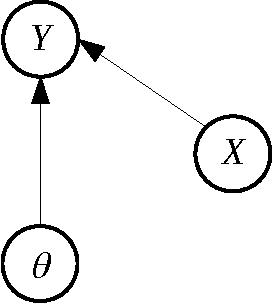
\includegraphics[width=.25\textwidth]{generative.pdf}\label{fig:generative}}
\hspace*{.2\textwidth}
\subfigure[Discriminative model]{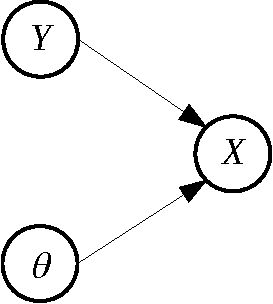
\includegraphics[width=.25\textwidth]{discriminative.pdf}\label{fig:discriminative}}
\caption{Directed graphs representing a generative and discriminative models, where $X$, $Y$ and $\theta$ respectively denote the target variable, the data, and the model parameters. Note the marginal independence of data and parameters in the discriminative model.}
\label{fig:graph_comparison}
\end{center}
\end{figure}

This note advocates probabilistic opinion pooling \cite{Genest-86} as a natural way to merge discriminative and generative modeling approaches in order to make predictions that are both accurate and interpretable. The key idea is to combine multiple low-dimensional generative models corresponding to different pieces of information extracted from the input data. Each such model acts as an isolated ``agent'' that uses a single feature to express a testable opinion in the form of a likelihood function of the target variable. The agent opinions are then aggregated into a unique predictive probability distribution analogous to a Bayesian posterior. This idea may be understood as a probabilistic version of boosting, or as a ``divide and conquer'' approximation to the intractable Bayesian posterior. 

%Importantly, each agent opinion is justifiable as it is based on a generative model.

When choosing the aggregation method as log-linear pooling, the predictive distribution turns out to be proportional to a quantity known in computational statistics as composite likelihood (CL), see \cite{Varin-11} and the references therein. CL was developed as a surrogate of traditional likelihood for parameter estimation. While maximum CL does not inherit the general property of maximum likelihood to achieve asymptotical minimum variance, it is asymptotically consistent under mild conditions \cite{Xu-11} (see Appendix~\ref{app:frequentist} for a basic weak consistency proof), and may offer an excellent trade-off between computational and statistical efficiency in practice.

Following the opinion pooling interpretation, the weights assigned to the different features in~CL may be optimized for prediction performance in a typical supervised learning scenario. As we will see, this strategy amounts to training a maximum entropy classifier using the feature-based log-likelihoods as basis functions. The likelihood functions themselves may need to be pre-trained, therefore the composite Bayesian approach typically involves a two-stage training scheme: a generative training (to learn the feature-based likelihood parameters) followed by a discriminative training (to learn the feature weights in aggregation).

The opinion pooling framework also suggests a generalization of CL, which we call {\em super composite likelihood}, in which the features may be weighted depending on the target values, leading to a more flexible predictive model that can be trained similarly.

%Technical details are given in the remainder. 

The reader is warned that slightly abusive mathematical notation is sometimes used in the remainder. This is done deliberately for the sake of clarity in places where we think that notation can be lightened without ambiguity. 


\section{Composite likelihood as opinion pooling}
\label{sec:log_pool}

Let $\mathbf{Y}$ an observable multivariate random variable with sampling distribution $p(\y|x)$ conditional on some unobserved variable of interest, $X\in{\cal X}$, where ${\cal X}$ is assumed to be a finite set for simplicity. Given an experimental outcome $\y$, the likelihood is the sampling distribution evaluated at $\y$, seen as a function of $x$:
$$
L(x) = p(\y|x).
$$

This requires a plausible generative model which, for complex data, may be out of reach or involve too many nuisance parameters. A natural workaround known as data reduction is to extract some lower-dimensional representation $z(\y)\sim f(z|x)$ using a many-to-one mapping, and consider the potentially more convenient likelihood function:
$$
\ell(x) = f(z|x).
$$

Substituting $L(x)$ with $\ell(x)$ boils down to restricting the feature space, thereby  ``delegating'' statistical inference to an ``agent'' provided with partial information. While it is valid for such an agent observing~$z$ only to consider $\ell(x)$ as the likelihood function of the problem, the drawback is that $\ell(x)$ might yield too vague a prediction of~$X$ due to the information loss incurred by data reduction. To make the trick statistically more efficient, we may extract several features, $z_i(\y)$ for $i=1,2,\ldots,n$, and try to combine the likelihood functions $\ell_i(x) = f(z_i|x)$ that they elicit.

If we see the likelihoods as Bayesian posterior distributions corresponding to {\em uniform} priors, this is a problem of probabilistic opinion aggregation from possibly redundant sources, for which several methods exist in the literature \cite{Tarantola-82,Genest-86,Garg-04,Allard-12}. One that is simple and satisfies a much desirable unbiasedness property is log-linear pooling\footnote{When $\pi(x)$ is not uniform, it is also called {\em generalized} log-linear pooling, however this terminology could be confusing here since we will present another generalization.}:
\begin{equation}
\label{eq:log_pool}
p_\blambda(x|\y) \propto \pi(x) \prod_{i=1}^n f(z_i|x)^{\lambda_i},
\end{equation} 
where $\pi(x)$ is a reference distribution and $\blambda=(\lambda_1,\ldots,\lambda_n)$ is a vector of weights. Log-linear pooling is {\em unbiased} in the sense that eliminating some hypotheses does not alter the probability ratios between the remaining hypotheses (see Appendix~\ref{app:log_pool_standard}). We shall asume for feasibility that the weights are intrinsic to the agents and are therefore independent from the data~$\y$. Also, negative weights should be ruled out to warrant a natural monotonicity property: if all agents agree that an hypothesis $x_1$ is less probable than an hypothesis $x_2$, this should be reflected by the consensus probabilities, {\em i.e.}, we should have $p_\blambda(x_1|\y)\leq p_\blambda(x_2|\y)$. As a convenient effect of using positive weights, log-linear pooling tends to produce single peaked distributions.


\section{Composite Bayes rule}
\label{sec:bayes_rule}

Log-linear pooling~(\ref{eq:log_pool}) bears a striking similarity to Bayes rule as it yields the form: 
$$
p_\blambda(x|\y)\propto \pi(x) L^c_\blambda(x),
$$
where the distribution $\pi(x)$ plays the role of a prior, while the quantity:
\begin{equation}
\label{eq:comp_lik}
L^c_\blambda(x) \equiv \prod_{i=1}^n \ell_i (x)^{\lambda_i}
\end{equation} 
plays that of a likelihood function, and happens to be known in computational statistics as a {\em marginal composite likelihood} \cite{Varin-11}. The slightly more general {\em conditional composite likelihood} form can be derived in the same way as above by conditioning all probabilities on confounding variables, see Appendix~\ref{app:conditional}. 

The clear computational advantage of CL over genuine likelihood is that it is more efficient to evaluate the marginal distributions of each feature than the joint distribution of all features. CL shares a convenient factorized form with the likelihood derived under the assumption of mutual feature independence, often referred to as {\em na\"ive Bayes} method in the machine learning literature, which corresponds to the special case of unitary weights, $\blambda\equiv 1$. Since log-linear opinion pooling does not assume feature independence, it yields both an alternative interpretation and a generalization of na\"ive Bayes, whereby unitary feature weights may be used by default but do not guarantee optimal prediction performance.


\section{Composite likelihood calibration}
\label{sec:calibration}

CL involves two types of parameters:
\begin{enumerate}
    \item ``generative'' parameters, {\em i.e.}, the parameters of the feature generation models $f(z_i|x)$; 
    \item ``discriminative'' parameters, {\em i.e.},  the weights~$\blambda=(\lambda_1,\ldots,\lambda_n)$ assigned to the feature-based likelihood functions in~(\ref{eq:log_pool}).
\end{enumerate}

If training data is available, the generative parameters may be tuned in a first stage using standard estimation techniques. Otherwise, they may be considered as nuisance parameters and eliminated at prediction time by applying to CL one of the same techniques as for traditional likelihood \cite{Berger-99}. We focus in the sequel on tuning the composite weights.


\subsection{Agnostic weights}

In the absence of knowledge, uniform weights may be chosen under a rule of indifference. CL is then a scaled version of na\"ive Bayes likelihood, the unique weight value being irrelevant to the maximum CL estimator (MCLE). To get meaningful predictive probabilities, it may be tuned empirically so as to best adjust the pseudo posterior variance matrix to the asymptotic MCLE variance matrix \cite{Pauli-11}, or via a close-in-spirit curvature adjustment \cite{Ribatet-12}, as proposed in previous attempts at Bayesian inference from composite likelihood. 

Alternatively, a simple agnostic recommendation we believe to be useful for composite weights is to sum up to one. This is motivated by a characterization theorem \cite{Genest-86,Genest-86b}: the only {\em externally Bayesian} pooling operator for which the consensus probability of an outcome only depends on the agent probabilities of the same outcome, is log-linear opinion pooling constrained to unit sum weights. The external Bayesian property is stronger than the above-mentionned unbiasedness property; it essentially means that the consensus should not change if any agent opinion is taken into account by the other agents as opposed to being stated independently. Log-linear pooling with unit sum weights also turns out to be an optimal {\em compromise} in the sense that it minimizes the average inclusive Kullback-Leibler (KL) divergence to the agent opinions \cite{Garg-04}. 

Unit sum weights, however, implicitly assume maximum redundancy between features, hence tend to produce conservative predictive probabilities (see Appendix~\ref{app:frequentist}). This means low prediction confidence (over-estimated credibility sets) when features are weakly correlated, as is desirable in general. Conversely, unitary weights ($\blambda\equiv 1$) as in Na\"ive Bayes assume independent features and may thus yield over-confident predictions. An ideal method to weight features is one that can capture feature redundancy and balance it with feature relevance \cite{Peng-05}. This suggests a learning approach whenever feasible.


\subsection{Learning the weights}
\label{sec:learning}

Assuming a training dataset ${\cal D}=\{(x_k,\y_k), k=1,\ldots,N\}$ (possibly the same as for generative pre-training), the most direct way to learn the composite weights is to maximize their likelihood under the composite predictive distribution or, equivalently, minimize prediction ``cross-entropy'':
\begin{equation}
\label{eq:train_likelihood}
\max_{\blambda\succeq 0} U(\blambda),
\qquad \text{with} \quad
U(\blambda) \equiv\sum_{k=1}^N \log p_\blambda(x_k|\y_k).
\end{equation}

From~(\ref{eq:log_pool}), we see that the set of conditional distributions $p_\blambda(x|\y)$ spanned by the weights~$\blambda$ is the exponential family with natural parameter~$\blambda$ and basis functions given by the feature-based log-likelihoods:
$$
p_\blambda(x|\y) = \pi(x) \exp[\blambda^\top \bell(x,\y) - a(\blambda,y)],
$$
with:
$$
\ell_i(x,\y) \equiv \log f(z_i|x),
\qquad
a(\blambda, \y) \equiv \log \sum_{x\in{\cal X}} \pi(x) e^{\blambda^\top \bell(x,\y)}.
$$

It follows that the utility function $U(\blambda)$ in~(\ref{eq:train_likelihood}) is concave as a general property of likelihood in exponential families, hence this learning can be implemented using a standard convex optimization algorithm such as limited-memory BFGS \cite{Byrd-95}. See Appendix~\ref{app:training} for some implementation details. 

Because some positive weight constraints may turn out inactive, optimization has a natural tendency to produce sparse weights. As illustrated in Figure~\ref{fig:disc_weight_plot} on the breast cancer diagnostic UCI dataset \cite{Wolberg-94}, there is no clear relation between optimal weights and feature-level discrimination power, showing that maximum likelihood learning differs radically from univariate feature selection as it implicitly takes feature redundancy into account via joint weight optimization.

\begin{figure}[!ht]
  \begin{center}
    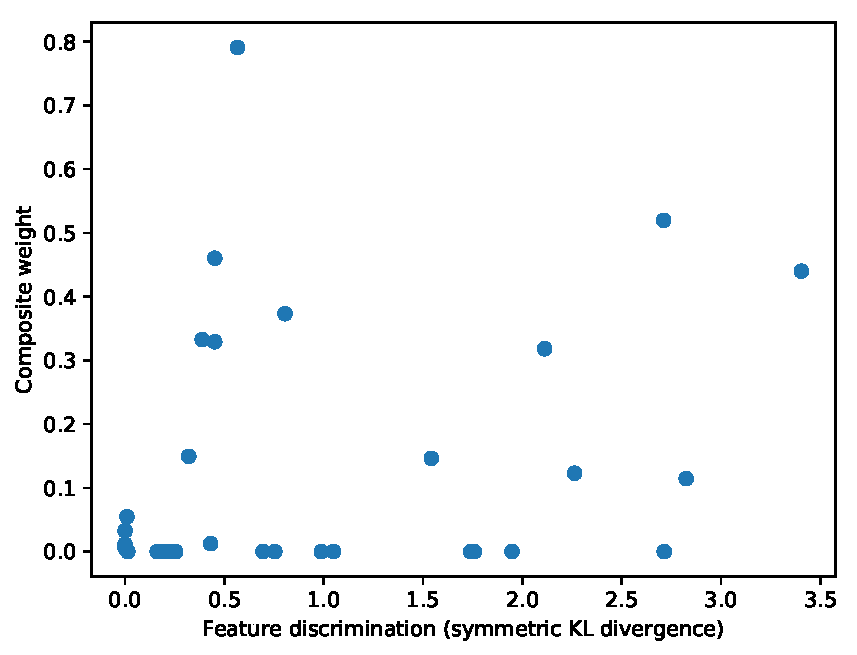
\includegraphics[width=.7\textwidth]{disc_weight_plot.pdf}
  \end{center}
\caption{Distribution of optimal composite weights vs.~individual feature discrimination power in a binary classification task (breast cancer UCI dataset). Discrimination is measured by the maximum KL divergence between class-conditional generative distributions.}
\label{fig:disc_weight_plot}
\end{figure}

As is customary and generally good practice, the training examples may be weighted in~(\ref{eq:train_likelihood}) so that the empirical distribution of classes matches the prior~$\pi(x)$, thus enforcing balanced classes if the prior is uniform. Also, some regularization may be needed for stability: we shall in practice maximize $U(\lambda)-\alpha \|\blambda\|^2$, where $\alpha>0$ is a small damping factor.

Other training variants that we mention here but do not particularly recommend for interpretability arise from adding basis functions to the exponential family. For instance, class-dependent offsets may be added so as to learn the ``prior'' together with the composite weights. It is also possible to perform unconstrained optimization to achieve higher training likelihood, but this means that some composite weights are then negative, in violation of the monotonicity property mentionned in Section~\ref{sec:log_pool}.


\paragraph{$I$-projection interpretation.}

Exponential family properties also imply that learning via likelihood maximization~(\ref{eq:train_likelihood}) is dual to an $I$-projection \cite{Csiszar-84}: 
\begin{equation}
\label{eq:i_proj}
\min_{p\in{\cal P}} D(p\|p_0),
\qquad \text{with} \quad
p_0(x,\y) \equiv \pi(x)h(\y),
\end{equation}
subject to the constraints $p(\y)=h(\y)$ and $\E_p[\bell] \succeq \E_h[\bell]$, where $\E_h$ denotes the expectation with respect to the joint {\em empirical} distribution of targets and inputs, $h(\y)$ is the corresponding empirical marginal distribution of inputs, and ${\cal P}$ is the set of joint probability distributions on ${\cal X}\times {\cal Y}$ with ${\cal Y}\equiv\{\y_1,\ldots,\y_N\}$. Note that the problem statement implicitly approximates the true (unknown) joint distribution of $(x,\y)$ by its empirical estimate, hence the need for regularization in practice.

The marginal constraint $p(\y)=h(\y)$ implies that only the conditional distribution $p(x|\y)$ is optimized, making the $I$-projection equivalent to maximum conditional entropy \cite{BergerA-96}. The mean log-likelihood constraints $\E_p[\bell] \succeq \E_h[\bell]$ encapsulate dependences between the target and the data, and consider a model admissible if it guarantees the same average log-likelihood levels as observed separately for each feature. This is weaker a constraint than assuming that the feature generative models $f(z_i|x)$ are true: it only assumes that the {\em description length} \cite{Grunwald-07} achieved by each feature model is a truthworthy upper bound. The composite likelihood weights may be interpreted as the Lagrange multipliers associated with these description length constraints. 

An insightful analysis given in \cite{Grunwald-04} shows that $I$-projection is, under broad conditions, a minimax strategy for prediction according to the log loss. Hence, any $I$-projection is in some sense a best possible predictive model given some arbitrary knowledge exctracted from the training data, which is represented by mean-value constraints and is {\em inexact} in practice due to the finite training set. Optimized composite likelihood only differs from other maximum entropy classifiers such as multinomial logistic regression by its underlying inexact knowledge, which in this case may be interpreted in terms of feature description length.


\section{Super composite likelihood}
\label{sec:super}

So far, we have assumed that each agent is given a single weight in the opinion aggregation~(\ref{eq:log_pool}). Let us now consider a more general pooling operator where agents can be weighted depending on the target variable:
\begin{equation}
\label{eq:super_pool}
p_\blambda(x|\y) \propto \pi(x) \prod_{i=1}^n \left[\frac{\ell_i(x)}{\ell_i(x_0)}\right]^{\lambda_i(x)},    
\end{equation}
where~$x_0$ is an arbitrary fixed target value, which we call the reference, and $\blambda: {\cal X}\to \mathbb{R}_+^n$ is a weighting function here. Note that the reference weights $\lambda_i(x_0)$ play no role and can therefore be conventionally assumed to cancel. As shown in Appendix~\ref{app:log_pool_hetero}, the main reason for introducing the normalization by a reference is to make pooling externally Bayesian if the weighting function sums up to one uniformly,
$$
\forall x\in{\cal X}\setminus \{x_0\},\quad
\sum_{i=1}^n \lambda_i(x) = 1,
$$
hence providing a sensible default rule to tune the weights. Note that (\ref{eq:super_pool}) amounts to log-linear pooling if the weights are target-independent as the reference is then effectless. Using the same analogy with Bayes rule as in Section~\ref{sec:bayes_rule}, we see that the quantity:
\begin{equation}
\label{eq:super_comp_lik}
L^{sc}_\blambda(x) \equiv 
\prod_{i=1}^n \left[\frac{\ell_i(x)}{\ell_i(x_0)}\right]^{\lambda_i(x)}
\end{equation} 
acts as a likelihood function at prediction time. We call the form~(\ref{eq:super_comp_lik}) super composite likelihood (SCL) owing to the ``doubly composite'' aspect of combining distinctive feature-target pairs. SCL further generalizes CL since both forms are seen to be proportional for target-independent weights. 

Conversely, if the weighting function maps each target to a unit vector ({\em i.e.}, $\forall x\in{\cal X}\setminus \{x_0\}$, $\lambda_i(x)=1$ for a single feature~$i$, and zero otherwise), then SCL turns out identical to the class-specific likelihood surrogate derived in \cite{Baggenstoss-03} from a generative model selection argument; namely, the {\em PDF projection theorem}, which in fact boils down to an $I$-projection \cite{Minka-04}. While our derivation follows a {\em discriminative} model selection approach, it is interesting to see that it includes the class-specific method as a special case, and thus sheds new light on this method.

A compelling advantage of SCL over CL is that it can deal with missing likelihood values, which happen if the feature generative distributions $f(z_i|x)$ are unknown for some targets~$x$. SCL makes it possible to assign zero weights $\lambda_i(x)$ to every feature-target pair for which $\ell_i(x)$ is unknown, yet using nonzero weights for other pairs. Likewise, the features for which the reference likelihood $\ell_i(x_0)$ is unknown receive zero weight for all target values, implying that they have no influence whatsoever on the predictive distribution.

If training data is available, the SCL weights may be learned by maximum likelihood as described for CL in Section~\ref{sec:learning}, yielding a similar convex problem. Since SCL enables to explore a wider class of predictive models than CL, it has the potential to achieve better prediction performance as long as overfitting does not happen during training (although SCL may not be asymptotically consistent unlike CL, see Appendix~\ref{app:frequentist}). The $I$-projection interpretation still holds, yet with class-specific mean-value constraints:
$$
\forall a\in{\cal X}, \forall i=1,\ldots,n,
\quad
\E_p\left[\delta_{xa}\log \frac{f(z_i|x)}{f(z_i|x_0)}\right]
\geq \E_h\left[\delta_{xa}\log \frac{f(z_i|x)}{f(z_i|x_0)}\right],
$$
where $\delta$ denotes the Kronecker delta. 




\section{Discussion}
\label{sec:discussion}

The composite Bayesian framework unifies several seemingly unrelated concepts from computational statistics and machine learning: composite likelihood \cite{Varin-11}, PDF projection \cite{Baggenstoss-03}, na\"ive Bayes. It ultimately provides a rich class of trainable predictive models that work on pre-determined data features, and is therefore suitable for ``shallow'' learning tasks, where it may compete with classical discriminative models such as logistic regression, support vector machines or random forests. Potential use cases include transfer learning \cite{Goodfellow-16}, {\em i.e.}, when features are learned automatically in a related task via deep learning, for instance.

Unlike previous attempts at Bayesian inference from incomplete statistical models that relied on generative model selection \cite{Yuan-99b,Wang-14} or asymptotic theory \cite{Pauli-11,Ribatet-12}, our construction is based on a discriminative model selection approach. Composite Bayesian models are thus explicitly taylored to prediction and cannot simulate complete data but, contrary to conventional discriminative models, they encapsulate feature generation models.

Training a composite Bayesian model involves the sequential estimation of feature generative parameters and feature relevance weights. This two-stage training is reminiscent of restricted Boltzmann machines (RBMs) \cite{Hinton-06,Fischer-14}, which are fully generative models, with the important difference that it operates on {\em disjoint} sets of parameters in the case of composite Bayesian models, while RBM training modifies the same parameters twice. Also, the generative training stage of RBMs is typically unsupervised, and it is an open research issue whether composite Bayesian models are suitable for unsupervised learning.

\begin{figure}[!ht]
\begin{center}
\subfigure[Case study: clearly categorized class-3 wine]{
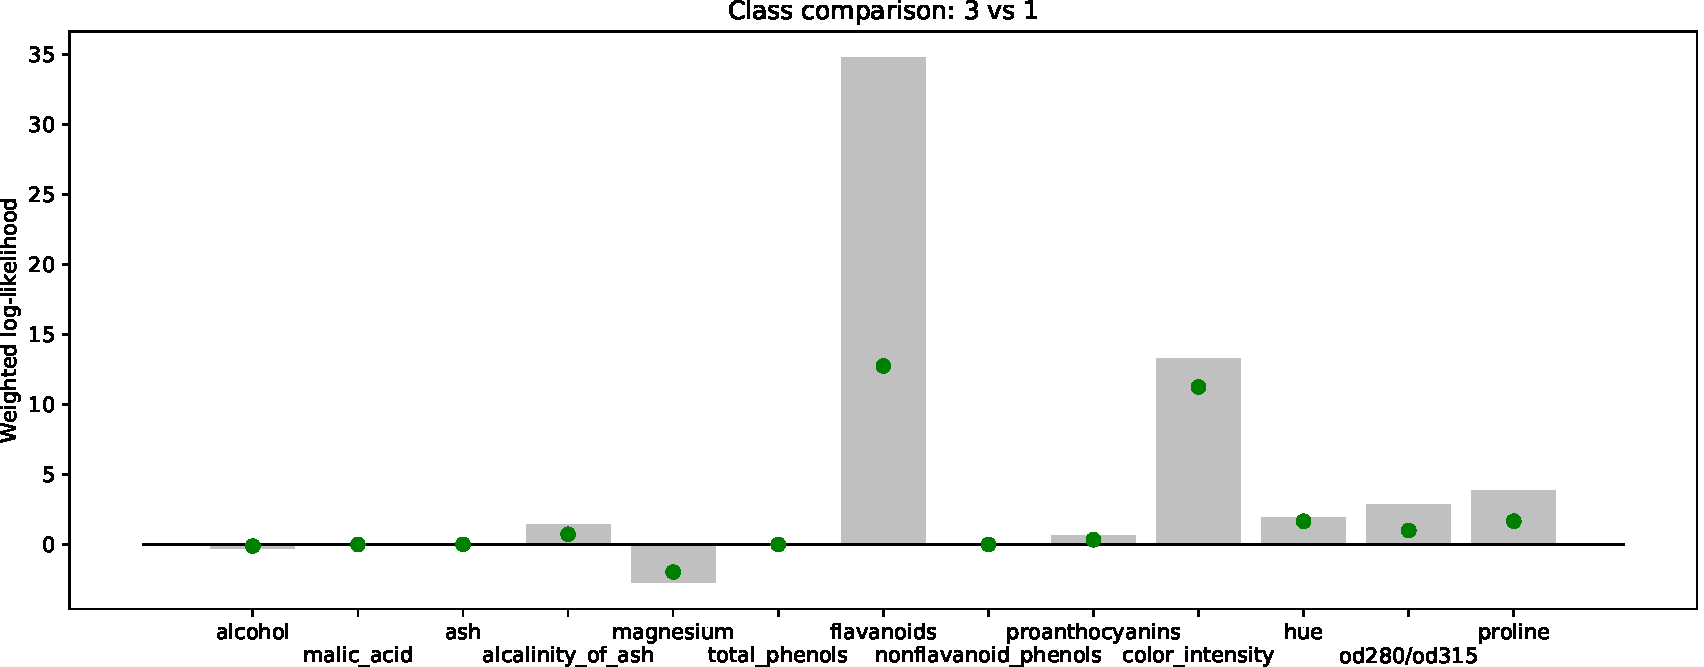
\includegraphics[width=.9\textwidth]{interp_case1.pdf}}
%\hspace*{.2\textwidth}
\subfigure[Case study: atypical class-2 wine]{
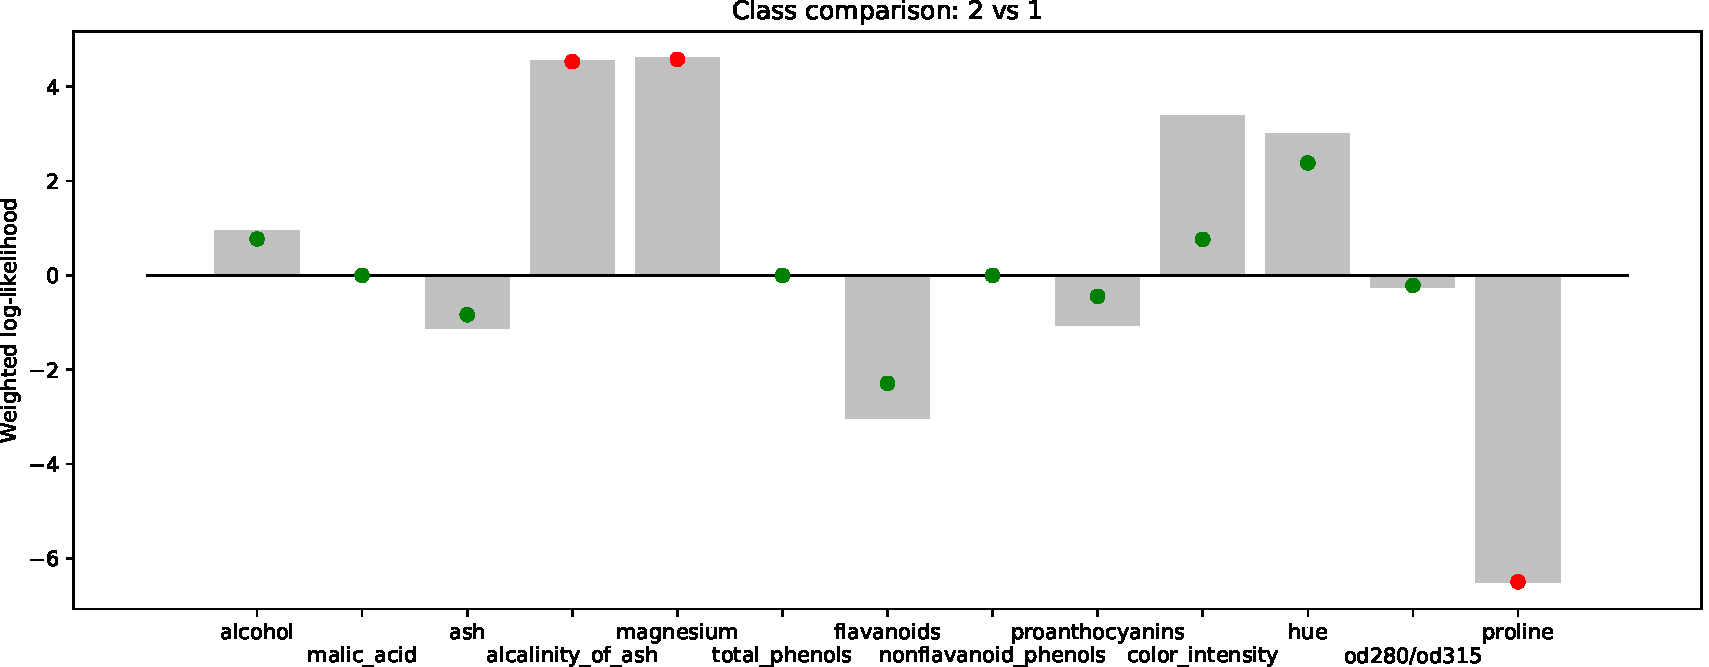
\includegraphics[width=.9\textwidth]{interp_case2.pdf}}
\end{center}
\caption{Graphical representation of feature influence on wine classification in a composite Bayesian model using heteroscedastic Gaussian feature generation models and uniform prior. Bars represent feature contributions to the difference of log-composite likelihoods between the most probable and second most probable class. Dots represent $\chi^2$ feature percentiles under the most probable class; green and red colors mark values respectively smaller and larger than 95\%.}
\label{fig:interp}
\end{figure}

Interpretability is from our point of view the key advantage of composite Bayesian models. It results from their semi-generative nature, which enables to test at prediction time how consistent the input data is with each feature distribution, thereby providing the user with crucial clues to understand and validate the prediction. Moreover, since feature log-likelihoods are combined additively, it is easy to determine which features contribute most to a particular comparison of hypotheses about the target, and summarize the rational for a prediction by highlighting a few decisive features. 

This is illustrated in Figure~\ref{fig:interp} for a composite Bayesian expert fully trained (including weight optimization as in Section~\ref{sec:learning}) on a famous UCI dataset \cite{Aeberhard-92} to classify wines into 3 categories from 13~features. The top panel shows how the expert (correctly) classifies a particular wine in category~3 with near $100\%$ probability; it can be seen that the prediction is mainly based on the flavanoids concentration and the color intensity. Since both have typical values for category~3 wines, this is a clear-cut decision. In another case depicted in the bottom panel, the wine is (again, correctly) classified in category~2 with $98.9\%$ probability, however two of the main features driving the prediction (alcanality of ash and magnesium concentration) have peculiar values for category~2, while proline concentration quite strongly points to category~1. Despite high prediction confidence, this case may require further investigation.

We believe that there are many applications of statistical inference in which interpretation is the real goal while prediction performance is only an intermediate requisite. A prediction method needs to prove reliable to be relevant; but, once proven reliable, it may need to be interpreted. Composite Bayesian inference may come into play when the {\em why} question is more important than the {\em what} question.


\appendix


\section{Basic frequentist properties of composite likelihood}
\label{app:frequentist}

Let a multivariate observable variable~$\y \sim p(\y|x_\star)$ distributed according to some target value~$x_\star$. For any hypothetical target value~$x$ and any extracted feature $z_i\sim f(z_i|x)$, the following double inequality holds:
$$
0 \leq
E\left[
\log \frac{f(z_i|x_\star)}{f(z_i|x)}
\right]
\leq
E\left[
\log \frac{p(\y|x_\star)}{p(\y|x)}
\right],
$$
where the expectation is taken with respect to the true distribution $p(\y|x_\star)$ at fixed~$x_\star$. This fact follows from two basic properties of KL~divergence: positivity and partition inequality.

Using a weighted sum of such inequalities, we can bracket the expected variations of the logarithm of any composite likelihood function~(\ref{eq:comp_lik}) using positive weights~$\blambda\succeq 0$:
\begin{equation}
\label{eq:variation_bound}
0 \leq
E\left[ \log \frac{L_c(x_\star, \blambda)}{L_c(x,\blambda)} \right]
\leq 
\|\blambda\|_1 E\left[ \log \frac{L(x_\star)}{L(x)} \right]
,
\end{equation}
where $\|\blambda\|_1 =\sum_i \lambda_i$ and $L(x)\equiv \log p(\y|x)$ is the true likelihood function. This trivially implies two general asymptotic properties of composite likelihood:
\begin{itemize}
\item {\em Weak consistency.} The expected composite log-likelihood is maximized by~$x_\star$.
\item {\em Conservativeness.} If the weights sum up to one or less ($\|\blambda\|_1\leq 1$), composite likelihood ratios of the true target~$x_\star$ vs.~other target values~$x$ tend to  underestimate true likelihood ratios.
\end{itemize}

Note that the derivation assumes that the weights~$\blambda$ are independent from the target~$x$, therefore these properties do not necessarily extend to SCL.


\section{Conditional composite likelihood}
\label{app:conditional}

As a straightforward  extension of marginal CL, each feature-based likelihood may be conditioned by an additional ``independent'' feature $\nu_i(\y)$ considered as a predictor of the ``dependent'' feature, $z_i(\y)$, yielding the more general form:
\begin{equation}
\label{eq:cond_feat_lik}
\ell_i(x) = f(z_i|x,\nu_i).
\end{equation}

Conditioning may be useful if it is believed that $\nu_i$ alone provides little or no information about~$x$, but is informative when considered jointly with~$z_i$, as in the case of regression covariates, for instance. Equation~(\ref{eq:comp_lik}) then amounts to conditional CL \cite{Varin-11}, a more general form of CL which also includes Besag's historical {\em pseudo-likelihood} \cite{Besag-74} developed for image segmentation.


\section{Composite likelihood training}
\label{app:training}

Using the same notation as in Section~\ref{sec:learning}, the likelihood function in~(\ref{eq:train_likelihood}) can be expanded as follows:
$$
U(\blambda) 
= \sum_{k=1}^N \left[
\log \pi(x_k) + \blambda^\top \bell(x_k, \y_k) - a(\blambda,\y_k)
\right]
$$

Maximizing $U(\blambda)$ is therefore equivalent to maximizing: 
$$
\psi(\blambda) \equiv \blambda^\top \bar{\bell} - \bar{a}(\blambda), 
$$
with:
$$
\bar{\bell} \equiv \frac{1}{N} \sum_k \bell(x_k,\y_k),
\qquad
\bar{a}(\blambda) \equiv \frac{1}{N} \sum_k a(\blambda,\y_k).
$$

Note that $\psi(\blambda)$ is nothing but the dual function associated with the $I$-projection problem~(\ref{eq:i_proj}). The derivatives of~$\psi(\blambda)$ are found to be:
\begin{eqnarray*}
\nabla\psi(\blambda)
 & = & \bar{\bell} - \frac{1}{N} \sum_k \nabla a(\blambda,\y_k), \\
\nabla\nabla^\top\psi(\blambda)
 & = & - \frac{1}{N} \sum_k \nabla \nabla^\top a(\blambda,\y_k),
\end{eqnarray*}
with:
$$
\nabla a(\blambda,\y) = \E_{\blambda}(\bell),
\qquad
\nabla \nabla^\top a(\blambda,\y) = {\rm Var}_{\blambda}(\bell),
$$
where $\E_{\blambda}$ and ${\rm Var}_{\blambda}$ respectively denote the expectation and variance with respect to $p_\blambda(x|\y)\propto \pi(x)\exp[\blambda^\top \bell(x,\y)]$ at fixed~$\y$. This shows that $a(\blambda,\y)$ is convex in $\blambda$ since the variance matrix is positive, which, in turn, proves the concavity of~$\psi$.



\section{Log-linear pooling}
\label{app:log_pool}

Consider a sequence of probability distributions $p_i(x)$, $i=1,\ldots,n$, representing multiple opinions on a variable of interest~$x\in{\cal X}$. The general goal of opinion aggregation is to define an operator $F(p_1,\ldots,p_n)$ that takes opinions as inputs and outputs a single distribution $p(x)$ representing a consensus.

\subsection{Standard log-linear pooling}
\label{app:log_pool_standard}

Log-linear pooling \cite{Genest-86} is one particular such operator:
$$
p(x)\propto \pi(x) \prod_{i=1}^n p_i(x)^{\lambda_i},
$$
where $\pi(x)$ is an arbitrary distribution and $\lambda_i\in\mathbb{R}$ are arbitrary weights. 

A key property of log-linear pooling is that probability ratios are stable under hypothesis elimination: if the opinions are restricted to any subset ${\cal X}_s\subset {\cal X}$, the consensus~$p_s$ on ${\cal X}_s$ verifies $p_s(x_1)/p_s(x_2)=p(x_1)/p(x_2)$ for any pair $(x_1,x_2)\in{\cal X}_s\times {\cal X}_s$. In other words, eliminating some hypotheses does not bias inference towards any of the remaining hypotheses.

Another way to look at this invariance property is to state that, for any boolean-valued function $q:{\cal X}\to \{0,1\}$, opinion pooling and opinion updating commute: 
\begin{equation}
\label{eq:external_bayesian}
F[N(q p_1), \ldots, N(q p_n)]
=
N[q F(p_1,\ldots, p_n)],
\end{equation}
where~$N$ denotes the normalization endomorphism of $\mathbb{R}_+^{\cal X}$:
$$
N(f)(x) = \frac{f(x)}{\sum_{x'\in{\cal X}} f(x')}
.
$$

Note that if (\ref{eq:external_bayesian}) holds for any nonvanishing positive valued function $q:{\cal X}\to\mathbb{R}^\star_+$,  the opinion pool is said to be {\em externally Bayesian}, which is thus a more general property than probability ratio invariance. It is easily seen that log-linear pooling is externally Bayesian if the weights~$\lambda_i$ sum up to one. Conversely, \cite{Genest-86b} proved that any externally Bayesian operator for which the consensus evaluated at~$x$, $F(p_1,\ldots,p_n)(x)$, is a function of $x,p_1(x),\ldots,p_n(x)$, is a log-linear opinion pool with unit sum weights. 

\subsection{Heterogeneous log-linear pooling}
\label{app:log_pool_hetero}

Log-linear pooling may not be ideal if agent have {\em selective} opinions in the sense that they respond more to certain outcomes  than to others. For instance, some agent may produce a sharply peaked distribution only when the target variable is in a certain state but a flat distribution otherwise, and some other agents may selectively respond to other states. In such situation, it is natural to try and weight agents depending on outcomes, so that $\lambda_i$ becomes a function of~$x$. 

As a first try, let us consider log-linear pooling in this scenario:
$$
p(x)\propto \pi(x) \prod_i p_i(x)^{\lambda_i(x)},
$$
where $\lambda_i : {\cal X}\to\mathbb{R}$ is now a weighting function. Unfortunately, this more general operator does not satisfy hypothesis reduction invariance. The reason 

It is easily seen that, if the weights sum up to one, log-linear pooling is externally Bayesian in the sense that, for any nonvanishing positive valued function $q:{\cal X}\to \mathbb{R}^\star_+$, opinion pooling and opinion updating commute:
$$
F[N(q p_1), \ldots, N(q p_n)]
=
N[q F(p_1,\ldots, p_n)],
$$
where~$N$ denotes the normalization endomorphism of $\mathbb{R}_+^{\cal X}$:
$$
N(f)(x) = \frac{f(x)}{\sum_{x'\in{\cal X}} f(x')}
.
$$

Conversely, \cite{Genest-86b} proved that any externally Bayesian operator for which the consensus evaluated at~$x$, $F(p_1,\ldots,p_n)(x)$, is a function of $x,p_1(x),\ldots,p_n(x)$, is of the above form with unit sum weights and is therefore a log-linear opinion pool. 

Log-linear pooling may not be ideal if agent opinions are {\em selective}. Assume, for instance, that some agent produces a sharply peaked distribution only when the target variable is in a certain state but a flat distribution otherwise, and that some other agents selectively respond to other states. In such situation where opinions reflect some outcomes better than others, it would be natural to try and weight agents depending on outcomes, so that $\lambda_i$ becomes a function of~$x$. 

As a first try, let us consider log-linear pooling in this scenario:
$$
p(x)\propto \pi(x) \prod_i p_i(x)^{\lambda_i(x)},
$$
where $\lambda_i : {\cal X}\to\mathbb{R}$ is now a weighting function. Unfortunately, this more general operator is not externally Bayesian:
$$
F[N(q p_1), \ldots, N(q p_n)](x)
\propto
\underbrace{q(x)^{\sum_i \lambda_i(x)} \prod_i z_i^{-\lambda_i(x)}}_{r(x)}
F(p_1,\ldots, p_n)(x),
$$
with:
$$
z_i \equiv \sum_{x\in{\cal X}} q(x) p_i(x),
$$
and the only way to make $r(x)$ proportional to $q(x)$ for any $q, p_1,\ldots, p_n$ is to impose constant weights, because the normalizing factors~$z_i$ may differ from one agent to the other.

Consider, however, the following alternative:
\begin{equation}
\label{eq:hetero_log_pool}
p(x) \propto \pi(x) \prod_i \left[\frac{p_i(x)}{p_i(x_0)}\right]^{\lambda_i(x)},    
\end{equation}
where $x_0$ is some arbitrary reference value. This does the trick because, for any positive function $q(x)$, the ratio $q(x)p_i(x)/q(x_0)p_i(x_0)$ is left unchanged by normalization of $q p_i$ since the normalizing factors are the same at both the numerator and the numerator, hence they cancel out, yielding:
$$
F[N(q p_1), \ldots, N(q p_n)](x)
\propto
\left[\frac{q(x)}{q(x_0)}\right]^{\sum_i \lambda_i(x)}
F(p_1, \ldots, p_n)(x),
$$
which shows that~(\ref{eq:hetero_log_pool}) is externally Bayesian whenever the weighting function verifies:
$$
\forall x \in {\cal X}\setminus \{x_0\},
\qquad
\sum_i \lambda_i(x) = 1.
$$

The operator~(\ref{eq:hetero_log_pool}) generalizes standard log-linear pooling and has the property that the consensus $F(p)(x)$ is a function of $x,p_1(x),\ldots,p_n(x)$ but also $p_1(x_0),\ldots,p_n(x_0)$. The ``trick'' to enable heterogeneous (target-dependent) weights is essentially to consider the odds relative to a fixed reference.

Caca.
$$
\log p(x) \equiv \mu(x) + \sum_i \lambda_i(x) \log p_i(x)
$$

If we look for a pool of the form:
$$
\log p(x) \equiv \mu(x) + \sum_i \lambda_i(x) \log p_i(x)
$$

However, log-linear pooling is not appropriate in situations where some agent opinions are not expressed on the whole set~${\cal X}$ of possibilities. Assume that the opinion~$p_i$ of agent~$i$ is only defined on a subset of~${\cal X}$: it could trivially be extended to~${\cal X}$ by assigning zero probability to missing outcomes, however that would mean that the probabilities provided by the agent are either underestimated or overestimated, and therefore unreliable.

In such situation, agent opinions somehow need normalization...

In such situation, it should be possible to weight opinions depending on target values, so that $\lambda_i$ becomes a function of~$x$.

have unreliable opinions about certain hypotheses. Assume, for instance, that an agent 

From this point on, only crap.

Ponderer les agents en fonction de $x$, c'est comme considerer des mini-agents ayant chacun une mini-opinion. Mais alors comment représenter ces mini-opinions? 

Une option est de choisir une fonction constante \'egale \`a $1$ sauf pour la cible particuliere du mini-agent, ou ca vaut $p_i(x)/p_i(x_0)$. Et là on fait du log-linear pooling. Sauf que ce n'est pas sur les opinions 'originelles'. Au passage, les mini-opinions n'ont pas besoin d'être normalisés. 

Du coup, on se ramene au log-linear pooling. La question est de savoir quelles strategies de construction de mini-agents sont acceptables. Opinions -> mini-opinions -> pooling.

Par exemple, si au lieu de prendre le rapport de proba, je prends juste $p_i(x)$ tout en laissant la ligne de base à 1, que se passe-t-il? On sent bien que c'est FOIREUX mais pourquoi? Ben, le rapport de proba n'est pas conserv\'e. Vu que la ligne de base est arbitraire, il faut d'une maniere ou d'une autre normaliser la valeur cible. 

Le mini-agent doit refleter un minimum l'agent dont il est issu. Conserver au moins un rapport de proba est une facon de garantir une certaine fidelite. 

Mais pourquoi conserver au moins un rapport? 



%\bibliographystyle{ieeetr}
\bibliographystyle{abbrv}
\bibliography{cvis,stat,alexis}

%%\documentclass[english]{scrartcl}

\usepackage{fullpage}
\usepackage{amstext,amssymb,amsmath,amsthm}
\usepackage{graphicx,subfigure}
\usepackage{multirow}
\usepackage{url}
\usepackage{hyperref}
\usepackage{color}

\graphicspath{{.}{pics/}}

%\newtheorem{theorem}{Theorem}[section]
%\newtheorem{proposition}[theorem]{Proposition}


\title{Composite Bayesian inference}
\date{}
\author{Alexis Roche\thanks{\url{alexis.roche@centraliens.net}}}

%\newcommand{\fix}{\marginpar{FIX}}
%\newcommand{\new}{\marginpar{NEW}}
%\newcommand{\matphi}{\boldsymbol{\Phi}} 
%\def\x{{\mathbf{x}}}
%\def\z{{\mathbf{z}}}
%\def\u{{\mathbf{u}}}
%\def\p{{\bar{\mathbf{p}}}}
%\def\q{{\bar{\mathbf{q}}}}



\begin{document}

\maketitle

\begin{abstract}
This note revisits the concept of composite likelihood from the perspective of probabilistic inference, and advocates a machine learning approach to tune the associated ``weights'', which stems naturally from a connection with the maximum entropy principle: the predictive distribution that maximizes conditional entropy relative to a given prior and subject to multiple mean log-likelihood inequality constraints is, up to a normalizing factor, the prior multiplied by a particular composite likelihood function, hence providing a ``composite'' extension of Bayes rule. We argue that composite Bayesian inference is a middle way between generative and discriminative approaches to statistical inference, which can be powerful in shallow learning and transfer learning problems.
\end{abstract}


\section{Introduction}
\label{sec:intro}

Classical frequentist and Bayesian inference paradigms rest upon the existence of a probabilistic data-generating model that is both empirically valid and computationally tractable. Because this is challenging for complex data, other inference models are commonly used in applied science: deliberately misspecified generative models, as in quasi-likelihood methods \cite{White-82,Walker-13} or na\"ive Bayes \cite{Ng-01}; data compression models as in minimum description length \cite{Grunwald-07}; and discriminative models\footnote{A {\em discriminative} model is a parametric family that describes the distribution of a variable of interest conditional on data, in contrast with a {\em generative} model, which describes the conditional distribution of data given the variable of interest.}, which currently dominate the field of artificial intelligence and typically require massive supervised learning -- these include classical techniques (maximum entropy classifiers \cite{BergerA-96}, support vector machines \cite{Vapnik-00}, Gaussian processes \cite{Rasmussen-06}) as well as most deep learning techniques \cite{Lecun-15,Goodfellow-16} with the exception of deep belief networks \cite{Hinton-06,Fischer-14}. 

A strong limitation of discriminative models is that they are not suitable for unsupervised learning or on-the-fly parameter estimation because they treat the data and the model parameters as {\em marginally independent}, meaning that the data conveys no information about the parameters unless the variable of interest is observed. This is illustrated in Figure~\ref{fig:graph_comparison} by the respective directed graph representations of generative and discriminative models. For the same reason, supervised learning in a discriminative model is less precise than in a generative model spanning the same family of posteriors, hence it is less effective in small training sets \cite{Ng-01}. Overall, pure discriminative models are of little use outside the context of big labeled data.

% p(x,y|theta) = p(x|y,theta)p(y|theta)

\begin{figure}[!ht]
\begin{center}
\subfigure[Generative model]{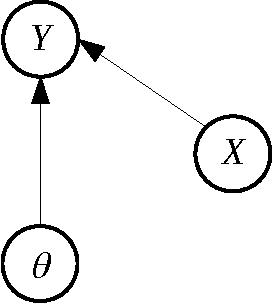
\includegraphics[width=.25\textwidth]{generative.pdf}\label{fig:generative}}
\hspace*{.2\textwidth}
\subfigure[Discriminative model]{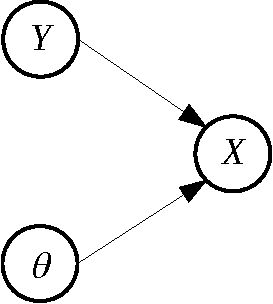
\includegraphics[width=.25\textwidth]{discriminative.pdf}\label{fig:discriminative}}
\caption{Bayesian networks representing generative and discriminative models, where $X$, $Y$ and $\theta$ respectively denote the variable of interest, the data, and the model parameters. Note the marginal independence of~$Y$ and~$\theta$ in the discriminative model.}
\label{fig:graph_comparison}
\end{center}
\end{figure}

Composite likelihood (CL, see \cite{Varin-11} and the references therein) is a semi-generative approach to statistical inference that extends the familiar notion of likelihood without requiring a full generative model. The key idea is to model an arbitrary set of low-dimensional features separately and then combine them, instead of modeling the data distribution as a whole. This may be viewed as a {\em divide and conquer} method to approximate the true but intractable likelihood. While maximum CL does not inherit the general property of maximum likelihood to yield an asymptotically minimum-variance estimator, it is consistent under mild conditions \cite{Xu-11} and may offer an excellent trade-off between computational and statistical efficiency in practice. 

In this note, CL is interpreted as a probabilistic opinion pool of ``agents'' making use of different pieces of information, or clues, extracted from the input data. Each agent acts as an isolated generative model-based statistician and expresses an opinion based on a single clue in the form of a likelihood function of the hidden variables. The agent opinions are then aggregated into a probability distribution on the hidden variables analogous to a Bayesian posterior.

We further argue that a particular log-linear opinion pool yields the best possible predictive distribution in the sense of maximum relative conditional entropy. This perspective entails a method to optimize the weights of the different agents from training data as in a typical discriminative learning scenario. 

%Something for true statisticians. Maybe we could clarify that we use the term ``Bayesian'' in the sense of ``empirical Bayesian'', implying that the parameters $\theta$ are to be estimated somehow contrary to a ``full Bayesian'' approach where they would be integrated out at inference time.


\section{Composite likelihood as opinion pooling}
\label{sec:pool}

Let $Y$ an observable multivariate random variable with sampling distribution $p(y|x)$ conditional on some unobserved variable of interest, $X\in{\cal X}$, where ${\cal X}$ is a known set. Given an experimental outcome $y$, the likelihood is the sampling distribution evaluated at $y$, seen as a function of $x$:
$$
L(x) = p(y|x)
.
$$

This requires a plausible generative model which, for complex data, may be out of reach or involve too many parameters to be estimated. A natural workaround known as {\em data reduction} is to extract some lower-dimensional representation $z=f(y)$, where $f$ is a many-to-one mapping, and consider the potentially more convenient likelihood function:
$$
\ell(x) = p(z|x)
.
$$

Substituting $L(x)$ with $\ell(x)$ boils down to restricting the sample space, thereby  ``delegating'' statistical inference to an ``agent'' provided with partial information. While it is valid for such an agent observing~$z$ only to consider $\ell(x)$ as the likelihood function of the problem, the drawback is that $\ell(x)$ might yield too vague a prediction of~$X$ due to the information loss incurred by data reduction. To make the trick statistically more efficient, we may extract several features, $z_i=f_i(y)$ for $i=1,2,\ldots,n$, and try to combine the likelihood functions $\ell_i(x) = p(z_i|x)$ that they elicit.

If we see the likelihoods as posterior distributions corresponding to uniform priors, this is a classical problem of probabilistic opinion aggregation from possibly redundant sources, for which several methods exist in the literature \cite{Tarantola-82,Genest-86,Garg-04,Allard-12}. We will show in Section~\ref{sec:maxent} that one that is particularly well-suited to our case is the {\em log-linear opinion pool}: 
\begin{equation}
\label{eq:log_pool}
p_\lambda(x|y) = \frac{1}{z_\lambda(y)} \pi(x) \prod_{i=1}^n p(z_i|x)^{\lambda_i},
\end{equation} 
where $\pi(x)$ is some reference distribution or prior, and $\lambda=(\lambda_1,\ldots,\lambda_n)$ is a vector of weights so that the normalizing factor:
$$
z_\lambda(y) = \int \pi(x) \prod_{i=1}^n p(z_i|x)^{\lambda_i} dx
$$
is finite, which holds whenever $\lambda\succeq 0$, {\em i.e.} all weights are positive, assuming that the agent opinions are always upper bounded. Negative weights should be ruled out as the existence condition $z_\lambda(y)<\infty$ would then depend on the particular opinions expressed by the agents. Also note that, while it is possible to have the weights depend on~$y$, there is a strong rational for constant weights as we shall see in the sequel. 

%Strictly positive weights guarantee the so-called 0/1 forcing property, that is, if an hypothesis~$x$ has zero likelihood according to at least one agent, then its consensus probability vanishes too.

% Not clear yet as to what a negative weight could mean!

The log-linear pool~(\ref{eq:log_pool}) bears a striking similarity to Bayes rule, yielding the form: $p_\lambda(x|y)\propto \pi(x) L^c_\lambda(x)$, where the quantity:
\begin{equation}
\label{eq:comp_lik}
L^c_\lambda(x) \equiv \prod_{i=1}^n \ell_i (x)^{\lambda_i}
\end{equation} 
plays the same role as a traditional likelihood function. This expression happens to be known in statistics as a {\em marginal composite likelihood} \cite{Varin-11}. See Appendix~\ref{sec:conditional} for the slightly more general form called {\em conditional composite likelihood}, which can be derived in the same way.

From~(\ref{eq:comp_lik}), we see that CL shares a convenient factorized form with the likelihood derived under the assumption of mutual feature independence, usually referred to as {\em na\"ive Bayes} or {\em simple Bayes} in the machine learning literature, which corresponds to the special case of unitary weights, $\lambda_1=\ldots=\lambda_n= 1$. The clear computational advantage of CL over the true likelihood is that it only requires to evaluate the marginal feature distributions rather than the joint distribution of all features.


\section{Tuning composite likelihood weights}

When the features can be considered exchangeable, it is natural to choose uniform CL weights. The CL is then a scaled version of the na\"ive Bayes likelihood, the common weight value being irrelevant to the maximum CL estimator (MCLE). The weight may be tuned so as to best adjust the pseudo posterior variance matrix to the asymptotic variance matrix of the MCLE \cite{Pauli-11}, or via a close-in-spirit curvature adjustment \cite{Ribatet-12}, in attempts to match the frequentist and composite Bayesian notions of uncertainty.

Ignoring such a goal, another frequent recommandation for CL weights is to sum up to one. This can be motivated in various ways. It turns out that the only pooling operator that does not explicitly depend on~$x$ and preserves {\em external Bayesianity} is the log-linear opinion pool with unit sum weights \cite{Genest-86b}. External Bayesianity essentially means that it should not matter whether the prior is incorporated before or after pooling, provided that all agents agree on the same prior. Another appealing property of log-linear pooling with unit sum weights is to minimize the average Kullback-Leibler (KL) divergence to the agent opinions \cite{Garg-04}. A maximum relative entropy property is also given in \cite{Wang-14}, Theorem~3.

Unit sum weights, however, correspond to the extreme situation where the features are assumed to be maximally redundant, but is clearly ineffective for independent or weakly correlated features, which require weights close to one for the CL to closely approximate the true likelihood. In this case, the CL may be much flatter than it should, leading to severly overestimated credibility sets.

{\color{red} Why is it important to fine-tune the weights?}
We therefore need a method to tune weights that can automatically adjust to the level of statistical dependence beween features.

%Instead, redundancy between agents is assumed by default, and is effectively encoded by the unit sum constraint on weights\footnote{Nevertheless, features which are {\em known} to be mutually independent can be merged into a single feature. This results in increasing their weights in the log-linear pool.}.

\section{Maxent composite likelihood}
\label{sec:maxent}

We can derive composite likelihood from the conditional maximum entropy principle \cite{BergerA-96}. It comes with a method of tuning weights, hence a particular composite likelihood function that we call maxent composite likelihood (MCL).

A cheap MaxEnt argument was already given by \cite{Wang-14}  (standard, non-conditional MaxEnt at fixed $y$, hence just an existence result but no feasible weight tuning).

What we do here is maximum {\em conditional} entropy. It's slightly more complex than a simple $I$-projection. The search space is a set of predictive distributions compatible with mean log-likelihood contraints. If I know the generative distribution, I know the expected log-likelihood.

We work with inequality constraints to force $\lambda\geq 0$:
$$
E[\log p(z_i|x)] \geq c_i \equiv \int \pi(x)p(z_i|x) \log p(z_i|x) dx dy
$$

What does the constraint mean? It means that a model is admissible if it compresses the data at least as well as all my agents. So we are not assuming that the generative models are {\em true}. We only assume that they are useful to compress the (reduced) data. Connection to MDL. 

Why not using the feature-based posteriors or Bayes factors rather than the likelihoods? It's a possibility (perhaps a connection here with Gr\"unwald's luckiness). A justification for not doing it is that the coordinator should discard the priors used by the agents. The constraints are not purely evidence-based since the moments depend on the coordinator's prior but it is arguable a mess of priors wouldn't be good.

Intuition behind weights: Lagrange multipliers to enforce a constraint... Notion of feature relevance. But does $\lambda_1>\lambda_2$ imply that $z_1$ is more relevant than $z_2$? 

The derivation assumed the marginal distribution of the data $h(y)$ to be known. In practice, it is estimated by the empirical distribution just like the moments are estimated.

Game theoretic interpretation \cite{Grunwald-04}.

The dual function boils down to the famous cross-entropy.

Single feature case ($y=z$): the maxent solution has the form $p(x|y)\propto\pi(x)p(y|x)^\lambda$. We expect to have $\lambda=1$ but it's not necessarily the case. It is if $h(y)=\int\pi(x)p(y|x)dx$ because then $h(y)p(x|y)=\pi(x)p(y|x)$ so the constraint is verified (and active). This also tells us that the data marginal should be consistent with the prior on labels for this much expected consistency property to hold. So, either weight datapoints so as to match a desired prior (e.g., uniform) or take the empirical distribution of labels as the ``prior''. 

Which brings another question: in this case, the (unique) weight is insensitive to the prior -- is it true in general? The answer is no. The weights generally depend on the prior. Hence the maxent composite likelihood is prior-dependent. This is an important conceptual difference with the classical notion of likelihood.

\section{Super composite likelihood}
\label{sec:super}

When chosen for computational simplicity, clues may not only convey limited information at individual level: their informativeness may also be very much hypothesis-dependent. Consider, for instance, diagnosing a disease from a routine medical checkup. Body temperature may point to a bacterial infection by comparison with normality, but would not help detecting a non-infectious cardiovascular disease -- and conversely for, say, blood pressure.

This motivates a more general setting where clues can be weighted differently depending on hypotheses.

What happens if we use mean-values constraints conditional on $x$ instead of jointly averaged over $x$ and $y$? This boils down to picking functions of the form:
$$
\chi(x-a)\ell_i(x,y)
$$

The answer is that the maxent solution has the form:
$$
p_\lambda(x|y) = \pi(x) \prod_i p(z_i|x)^{\lambda_i(x)}
$$

In other words, the weights become dependent on the variable of interest. This is the super composite likelihood idea.


\section{Composite EM algorithm for unsupervised learning}
\label{sec:gem}

In a nutshell: alternate unsupervised learning of partial model parameters ($M$-step) and re-estimation of label posteriors via maxent ($E$-step). 

$M$-step: given a posterior estimate $q(x|y)$, do just as if the features were independent and solve: 
$$
\max_\theta
\int \sum_i h(y)q(x|y) \log p_\theta(z_i,x) dx dy
$$

Note we can estimate cross-feature parameters such as class proportions.

Surrogate $E$-step: given generative parameters, recompute the moment constraints and update $q(x|y)$ according to the conditional maxent principle:
$$
\min_q
\int h(y)q(x|y) \log \frac{q(x|y)}{\pi(x)} dx dy
$$
s.t.
$$
\int h(y)q(x|y)\log p_\theta(z_i|x) dx dy \geq \int \pi(x)p_\theta(z_i|x)\log p_\theta(z_i|x) dx dy
$$

However, there is an important issue: how is $h(y)$ defined in both the $M$- and $E$-steps? In supervised context, $h(x,y)$ can be defined beforehand as the prior-corrected empirical distribution:
$$
h(x,y) = \pi(x) \frac{h_0(x,y)}{h_0(x)},
$$
where $h_0(x,y)$ is the raw empirical distribution. In unsupervised context, the best we can do is to replace $h_0(x,y)$ with $h_0(y)q(x|y)$, implying that the empirical distribution of $y$ is reweighted according to:
$$
h(y) = \sum_i w_i\delta(y-y_i),
\qquad
w_i = \int \pi(x)\frac{q(x|y_i)}{\sum_j q(x|y_j)} dx,
$$
which needs to be done each time $q(x|y)$ is updated, that is, after each $E$-step.

The other option is to keep $h(y)$ constant throughout the iterations but adapt $\pi(x)$ as the marginal distribution of labels learned in the $M$-step. In this case, it's no longer a ``prior''. 

Are we minimizing a unique functional as in the variational EM algorithm? Possibly not. We may see this generalization as a two-player game. One player tries to predict several data features independently. The other player tries to predict labels. Together, they find patterns (clusters) in unlabeled data. Does the more general version converge? Does the game have a value? And so on.

In the case of a single feature, is this the well-known EM? The $M$-step is clearly the same, what about the $E$-step? It is the same if $h(y)p_\theta(x|y)=p_\theta(y|x)\pi(x)$. However, this condition won't hold if $h(y)$ is an empirical distribution... In this special case, the ``E player'' could use the data distribution model produced by the ``M player'' instead of the empirical one but, more generally, there is no data distribution model so he has to stick to the empirical one.

The maxent is a surrogate for the $E$-step. It reflects the lack of a full model $p_\theta(x,y)$.

% Accounting here for Xi'An comment on xianblog.wordpress.com
% The sum of the powers is constrained to be equal to one, even though
% I do not understand why the dimensions of the projections play nog
% role in this constraint. Simplicity is advanced as an argument,
% which sounds rather weak…
%This simple constraint is implied by the external Bayesianity requirement: as it turns out, the only aggregation operator which is both externally Bayesian and independent from $x$ boils down to plugging a composite likelihood with unit sum weights into Bayes rule, hence extending the classical notion of likelihood in Bayesian analysis.


\section{Discussion}
\label{sec:discussion}

Deep learning is discriminative...

CL is a concept from computational statistics that has mainly been developed so far in a frequentist perspective as a surrogate for the maximum likelihood method. We have shown a deep connection between CL and probabilistic inference, thereby establishing CL as a class of discriminative models. Because CL is built from a set of marginal feature-specific generative distributions, it is in essence a two-step semi-generative, semi-discriminative learning approach. In the first, ``generative'' phase, the feature distributions are learned; in the second, ``discriminative'' phase, the feature weights are learned. This strategy can be thought of as a form of non-adaptive boosting.

%The first phase corresponds to the training of ``weak learners''. The second phase amounts to a form of boosting. 

A purely discriminative learning could be used instead but...
Why potentially more efficient than pure discriminative training: because generative training is always more efficient than discriminative training if models are comparable. So the key point is that ``we have less parameters in the discriminant phase". Good in small datasets. But also in asymptotic regime if the features are weakly or highly correlated (???).

Logistic regression / naive Bayes example. Under homoscedasticity (assuming that each feature has class-independent variance), CBI is equivalent to logistic regression -- because the predictive distribution family is the same. This is a case where BCI brings nothing. But consider heteroscedasticity, then BCI yields a quadratic classifier. Compared to a fully discriminative model, the number of parameters to learned in the discriminative phase is reduced by half.

The first training phase is easier if supervised but could be unsupervised too (using mixture models). How do we then deal with label switching issues? Can we safely assume conditional feature independence {\em in the generative training phase}? I believe so provided that the marginal distribution parameters are disjoint. It's obvious in the supervised learning scenario.

If unsupervised, the first learning phase could be compared with contrastive pre-training of RBMs \cite{Hinton-06,Fischer-14}, which also optimize parameters for generation of observable features. BCI is comparable with an RBM with a single output unit (which is just a generative model assuming conditionial feature independence). The key difference is that the RBM is a full generative model while BCI only deals with marginal models, hence relying on weaker assumptions. This won't change anything in the pre-training phase but RBMs have to deal with more parameters in the generative learning phase. In fully supervised context, RBM pre-training is pointless since all parameters learned in the first phase will be overwritten. In BCI, pre-training is crucial even in supervised context because the parameters learned in the discriminative phase (the feature weighs) describe a sub-manifold of the predictive distribution family.

Needs features. Not a representation learning method, but could be coupled why not.


%{\color{red} Moreover, while RBM parameters are typically refined in a supervised discriminative learning step, disjoint set of parameters for SCL. Dunno how to say that.} 

%In such context, SCL competes with classical discriminative models (logistic regression, Gaussian processes \cite{Rasmussen-06}, maximum entropy models \cite{BergerA-96}, etc.), and may compare more or less favorably in practice depending on the amount of training data. For relatively small training datasets, we may hope for more accurate inference using~SCL than using traditional discriminative models, extrapolating from the results of \cite{Ng-01} regarding the comparison between logistic regression and na\"ive Bayes classifiers.
%{\color{red}Ici, il manque la comparaison avec les RBMs qui ne sont pas (forcement) des modeles discriminatifs.}

%%, hence alleviating the need for heavily supervised model training

%In summary, CL has the potential to yield weakly supervised or unsupervised Bayesian-like inference procedures depending on the particular task at hand. This property reflects the encoding of statistical relationships between the data and {\em all} unknown parameters. CL thus appears as a trade-off between generative models, which are optimal for unsupervised learning but possibly intractable, and traditional discriminative models (logistic regression, Gaussian processes \cite{Rasmussen-06}, maximum entropy models \cite{BergerA-96}, etc.), which are inherently supervised. CL models are discriminative models assembled from atomic generative models and, from this point of view, may be considered as {\em semi-generative} models.

%CL may be considered as a {\em semi-generative} model: a discriminative model assembled from partial generative models.

%As a note of caution, we shall stress that the pre-determined weights assigned to the different associations between observed and unobserved values represent prior knowledge regarding the informativeness of clues. A poor choice of weights will inevitably result in a poor approximation to the ``true'' Bayesian posterior -- the posterior that would be obtained from a realistic generative model if it was tractable. In future work, we will investigate feature selection strategies to mitigate this problem.

% Improve the discussion on following aspects:
% ** Why is it compatible with unsupervised learning? Give more insight.
% ** Stress the contribution: class-specific weighting.
% * Pivotality argument.
% * Bayes is a special case of composite Bayes.

{\color{red}Product of fucking experts \cite{Hinton-02}. Log-linear pool to build a generative model (assuming in fact independence between experts). Better seen as a ``log-mixture model''. Sounds like each expert is associated with a class, so it's the same as a RBM. Contrastive learning approximates ML parameter estimation. The experts are learning jointly. It's just a generative model.}

{\color{red}Two-step training: generative phase then discriminative phase. Why is it cool?}

{\color{red}CBI is just a way to reweight Naive Bayes. What's the big deal? Can we really expect massively superior performance? Are we just talking about realistic credibility sets?}


\appendix

\section{Conditional composite likelihood}
\label{sec:conditional}

As a straightforward  extension of marginal CL, each feature-based likelihood may be conditioned by an additional ``independent'' feature $z^c_i = f^c_i(y)$ considered as a predictor of the ``dependent'' feature, $z_i=f_i(y)$, yielding the more general form:
\begin{equation}
\label{eq:cond_feat_lik}
\ell_i(x) = p(z_i|x,z^c_i).
\end{equation}

Conditioning may be useful if it is believed that $z^c_i$ alone is little or not informative about $x$, but can provide relevant information when considered jointly with $x$, as in the case of regression covariates, for instance. Equation~(\ref{eq:comp_lik}) then amounts to conditional CL \cite{Varin-11}, a more general form of CL also including Besag's historical {\em pseudo-likelihood} \cite{Besag-74} developed for image segmentation.


\section{Minimally discriminative model}

Let $\pi(x)$ some reference distribution that represents full
uncertainty about $X$. We wish to select the joint distribution
$p(x,y)$ that minimizes:
$$
I(p) = \int p(x,y) \log \frac{p(x|y)}{\pi(x)} dy,
$$ subject to feature mean-value constraints of the form:
$$
\int p(x,y) f(x,y) dx dy = \mu.
$$

There are two special cases of this problem in the literature.  On the
one hand, the {\em maximum entropy classifier} \cite{BergerA-96}
incorporates the constraint that $p(y)$ be known, however we will see
that this is not necessary. The {\em minimally informative likelihood}
method \cite{Yuan-99b,Yuan-99}, on the other hand, imposes that
$p(x)=\pi(x)$, hence assuming the form $p(x,y)=\pi(x)p(y|x)$. We won't
make such assumptions here and will consider the case where $\mu$ is
completely unknown.

The above problem is seen to be equivalent to minimizing the auxiliary
objective function:
$$
I(p,m) 
= \int p(x,y) \log \frac{p(x,y)}{\pi(x)m(y)} dxdy,
$$ over $p$ and $m$, subject to the same constraints on $p$. We note
that $I(p,m)=I(p)+D(p_y\|m)$, showing that the auxiliary function
essentially adds a penalty term to the actual objective in order to
force $p(y)$ close to $m(y)$.

Minimizing $I(p,m)$ along both $p$ and $m$ is basically a minimum KL
divergence problem between two convex distribution spaces, so there
must be a unique solution {\bf -- to be checked in
  \cite{Cover-91}}. It is similar to the rate-distortion problem in
information theory, which may be solved by alternate minimization,
yielding a Blahut-Arimoto algorithm.
\begin{itemize}
\item {\em Let's call it A-step}. Optimize $p(x,y)$ at fixed $m$
  s.t. constraint:
$$
\exists \lambda, \qquad
p_{\lambda,m}(x,y) = \frac{1}{Z(\lambda, m)} \pi(x) m(y) e^{-\lambda^\top t(x,y)}
$$
The actual $\lambda$ is found my maximizing the dual function
$\psi(\lambda,m)$, see below.
\item {\em Let's call it B-step}. Optimize $m(y)$ at fixed $p(x,y)$:
$$
m(y) = \int p(x,y) dx
$$
\end{itemize}

Upon convergence, the algorithm outputs both joint and marginal
distributions $p_{\star}(x,y)$ and $m_{\star}(y)$ that both depend on
$\mu$. By construction, we have that $p_{\star}(y) = m_{\star}(y)$,
therefore $p_\star(x|y)=p_{\star}(x,y)/m_{\star}(y)$.


\section{Comparison with maximum entropy classifier}

Lagrangian...
$$
{\cal L}(p,m,\lambda)
= 
\int p(x,y) \log \frac{p(x,y)}{\pi(x)m(y)} dxdy
+
\lambda^\top \left( 
\int p(x,y) f(x,y) dydy - \mu 
\right)
$$ where $\lambda$ represents a vector-valued Lagrange multiplier. At
fixed $m$, the solution has the form:
$$
p_{\lambda,m}(x,y) = \frac{1}{Z(\lambda,m)}
\pi(x) m(y) e^{-\lambda^\top f(x,y)} 
$$

Note that this implies that the conditional distribution is
independent of $m$ once $\lambda$ is determined,
$$
p_\lambda(x|y) = \frac{1}{z(\lambda,y)} \pi(x) e^{-\lambda^\top f(x,y)} 
$$

Also, the marginal is a modulation of $m(y)$:
$$
p_{\lambda,m}(y) = \frac{z(\lambda,y)}{Z(\lambda,m)} m(y)
$$

Dual function at fixed $m$:
$$
\psi(\lambda,m) 
\equiv \min_p {\cal L}(p,m,\lambda)
= 
- \log Z(\lambda,m) - \lambda^\top \mu
.
$$ 

An alternative expression is:
$$
\psi(\lambda, m)
= 
\int h(x,y) 
\log \frac{p_{\lambda,m}(x,y)}{\pi(x)m(y)} dxdy,
$$ where $h(x,y)$ is any distribution statisfying the
constraints. This shows that maximizing the dual function at fixed $m$
is essentially the same as minimizing the KL divergence
$D(h\|p_{\lambda,m})$ over $\lambda$, in other words fitting $h(x,y)$
by some distribution of the form $p_{\lambda,m}$. The fact that the
result does not depend on the particular $h(x,y)$ that is chosen, as
long as it satifies the constraint, is a general property of
exponential families.

We also have that the dual function associated with $I(p)$ reads:
\begin{eqnarray*}
\psi(\lambda) 
 & = & \min_m \psi(\lambda, m)\\
 & = & \int h(x,y) \log \frac{p_{\lambda}(x|y)}{\pi(x)} dxdy\\
 & = & -\int h(y) \log z(\lambda,y) dy - \lambda^\top \mu
\end{eqnarray*}

But, wait, that's exactly what we get in the maximum entropy
classifier! So, at the end of the day, we simply got an alternative
method to learn $\lambda$ in the maximum entropy classifier, i.e. the
Blahut-Arimoto algorithm as opposed to a brute-force maximization of
$\psi(\lambda)$. Both methods will converge to the same $\lambda$...

What it essentially means is that the optimal $\lambda$ is insensitive
to $m(y)$ as long as $m(y)$ is compliant in the sense that:
$$
m(y) = \int h(x,y) dx,
$$ for some distribution $h(x,y)$ statisfying the constraint. This is
true for the optimal $m_\star(y)$ output by the BA algorithm, but
also, for instance, for the empirical distribution of observations in
a training dataset used to estimate $\mu$, as proposed in
\cite{BergerA-96}. The only special property of $m_\star(y)$ is to
yield the full Bayesian model $p_\star(x,y)=p_\star(x|y)m_\star(y)$
that minimizes the discrimination information. We may not care too
much about that in practice since we will only use $p_\star(x|y)$. 

\section{Comparison with minimally informative likelihood}

Yuan \cite{Yuan-99} considered the situation where we add the
constraint that $p(x)=\pi(x)$ to the minimum discrimination inference
problem. Unknown is then the conditional distribution
$p(y|x)$. Lagrangian...
\begin{eqnarray*}
{\cal L}(p,m,\lambda)
 & = & 
\int \pi(x)p(y|x) \log \frac{p(y|x)}{m(y)} dxdy
+
\lambda^\top \left( 
\int \pi(x)p(y|x) f(x,y) dydy - \mu 
\right) \\
 & = & 
\int \pi(x)
\left( 
\int
p(y|x) \log \frac{p(y|x)}{m(y)} dy
+
\lambda^\top 
\int p(y|x) f(x,y) dy
- \mu 
\right)
dx 
\end{eqnarray*}

The derivative is given by,
$$
\frac{\partial\cal L}{\partial p(y|x)}
= 
\pi(x)\left[ 
1 + \log \frac{p(y|x)}{m(y)} 
+ \lambda^\top f(x,y)
\right],
$$
hence the optimal model at fixed $m$ has the form:
$$
p_{\lambda,m}(y|x) = \frac{1}{Z(\lambda,m,x)} m(y) e^{-\lambda^\top f(x,y)} 
$$

Note that the induced posterior distribution $p_{\lambda,m}(x|y)$ has
a different form from above unless the normalizing factor
$Z(\lambda,m,x)$ turns out independent from $x$. If this is not the
case, we no longer have the property that $p_{\lambda,m}(x|y)$ is
independent from $m$ given $\lambda$.

Dual function...
$$
\psi(\lambda,m) 
=
- \int \pi(x) \log Z(\lambda, m, x) dx
- \lambda^\top \mu
$$

Equivalently, for any distribution under the form $\pi(x)h(y|x)$ that
satisfies the moment constraint, we have:
$$
\psi(\lambda,m) 
=
\int \pi(x) h(y|x) \log \frac{p_{\lambda,m}(y|x)}{m(y)} dxdy
$$

Now, the real question is why should we constrain $p(x)$, which boils
down to a Bayesian prior in this context, to be the same as our
reference $\pi(x)$? It only makes sense if we want our inference to
stick to a generative modeling paradigm... but haven't we already
given up on that? Therefore, unless we find a good reason not to, we
won't impose the $p(x)=\pi(x)$ constraint, thereby allowing for a
discrepancy between the reference and the prior.


\section{Discriminative vs. semi-discriminative}

Let's go back to the equivalence we found between our approach and the
maximum entropy classifier (MCE) \cite{BergerA-96}. We have said that
the former is essentially a re-formulation of MCE.

But the re-formulation also conveys a generalization of MCE if,
instead of letting $m$ being an arbitrary distribution, we restrict
its search space to some set of acceptable reference
distributions. Would such a strategy be useful? 

Recall that the method selects the joint distribution that minimizes
discriminative information, as defined by $I(p)$:
$$
I(p) 
= \int p(x,y)\log\frac{p(x|y)}{\pi(x)} dxdy
= E_Y[D(p_{x|y}\|\pi)]
$$

The latter characterization reminds us that discriminative information
is defined in an average sense. The corresponding posterior $p(x|y)$
may not be conservative for some $y$, in particular those that are
unlikely under $p(y)$. It would be a problem if that's the case for
the particular data at hand. For that to happen rarely, the ideal
$p(y)$ would be the ``true'' marginal distribution of $Y$.

However, for vague mean value constraints, nothing may prevent the
optimal $m_\star(y)$ from departing significantly from that ideal
distribution. In fact, we can show that $m_\star(y)$ only has mass at
$y$ values that maximize $z(\lambda_\star,y)$, and is therefore likely
sparse. This is because $m_\star$ minimizes $\psi(\lambda_\star,m)$,
which is equivalent to maximizing $Z(\lambda_\star,m)$ and we have:
$$
Z(\lambda, m) = \int m(y) z(\lambda, y) dy.
$$

In other words, the solution to our problem may be singular! It does
not hurt since, as discussed above, one may alternatively fix $m(y)$
to some pre-defined distribution... but this, in practice, restricts
the method to supervised learning situations.

We may not face this issue with the MIL method, which further imposes
the prior on $X$, so all the information from the constraints goes
into specifying a possibly reasonable generative model.



\bibliographystyle{abbrv}
\bibliography{cvis,stat,alexis}

%%\documentclass[english]{scrartcl}

\usepackage{fullpage}
\usepackage{amstext,amssymb,amsmath,amsthm}
\usepackage{graphicx,subfigure}
\usepackage{multirow}
\usepackage{url}
\usepackage{hyperref}
\usepackage{color}

\graphicspath{{.}{pics/}}

%\newtheorem{theorem}{Theorem}[section]
%\newtheorem{proposition}[theorem]{Proposition}


\title{Composite Bayesian inference}
\date{}
\author{Alexis Roche\thanks{\url{alexis.roche@centraliens.net}}}

%\newcommand{\fix}{\marginpar{FIX}}
%\newcommand{\new}{\marginpar{NEW}}
%\newcommand{\matphi}{\boldsymbol{\Phi}} 
%\def\x{{\mathbf{x}}}
%\def\z{{\mathbf{z}}}
%\def\u{{\mathbf{u}}}
%\def\p{{\bar{\mathbf{p}}}}
%\def\q{{\bar{\mathbf{q}}}}



\begin{document}

\maketitle

\begin{abstract}
This note revisits the concept of composite likelihood from the perspective of probabilistic inference, and advocates a machine learning approach to tune the associated ``weights'', which stems naturally from a connection with the maximum entropy principle: the predictive distribution that maximizes conditional entropy relative to a given prior and subject to multiple mean log-likelihood inequality constraints is, up to a normalizing factor, the prior multiplied by a particular composite likelihood function, hence providing a ``composite'' extension of Bayes rule. We argue that composite Bayesian inference is a middle way between generative and discriminative approaches to statistical inference, which can be powerful in shallow learning and transfer learning problems.
\end{abstract}


\section{Introduction}
\label{sec:intro}

Classical frequentist and Bayesian inference paradigms rest upon the existence of a probabilistic data-generating model that is both empirically valid and computationally tractable. Because this is challenging for complex data, other inference models are commonly used in applied science: deliberately misspecified generative models, as in quasi-likelihood methods \cite{White-82,Walker-13} or na\"ive Bayes \cite{Ng-01}; data compression models as in minimum description length \cite{Grunwald-07}; and discriminative models\footnote{A {\em discriminative} model is a parametric family that describes the distribution of a variable of interest conditional on data, in contrast with a {\em generative} model, which describes the conditional distribution of data given the variable of interest.}, which currently dominate the field of artificial intelligence and typically require massive supervised learning -- these include classical techniques (maximum entropy classifiers \cite{BergerA-96}, support vector machines \cite{Vapnik-00}, Gaussian processes \cite{Rasmussen-06}) as well as most deep learning techniques \cite{Lecun-15,Goodfellow-16} with the exception of deep belief networks \cite{Hinton-06,Fischer-14}. 

A strong limitation of discriminative models is that they are not suitable for unsupervised learning or on-the-fly parameter estimation because they treat the data and the model parameters as {\em marginally independent}, meaning that the data conveys no information about the parameters unless the variable of interest is observed. This is illustrated in Figure~\ref{fig:graph_comparison} by the respective directed graph representations of generative and discriminative models. For the same reason, supervised learning in a discriminative model is less precise than in a generative model spanning the same family of posteriors, hence it is less effective in small training sets \cite{Ng-01}. Overall, pure discriminative models are of little use outside the context of big labeled data.

% p(x,y|theta) = p(x|y,theta)p(y|theta)

\begin{figure}[!ht]
\begin{center}
\subfigure[Generative model]{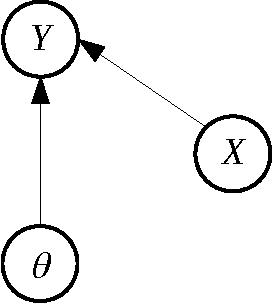
\includegraphics[width=.25\textwidth]{generative.pdf}\label{fig:generative}}
\hspace*{.2\textwidth}
\subfigure[Discriminative model]{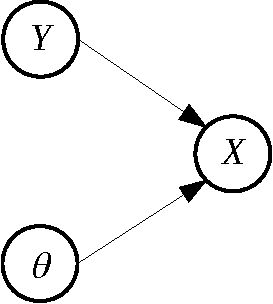
\includegraphics[width=.25\textwidth]{discriminative.pdf}\label{fig:discriminative}}
\caption{Bayesian networks representing generative and discriminative models, where $X$, $Y$ and $\theta$ respectively denote the variable of interest, the data, and the model parameters. Note the marginal independence of~$Y$ and~$\theta$ in the discriminative model.}
\label{fig:graph_comparison}
\end{center}
\end{figure}

Composite likelihood (CL, see \cite{Varin-11} and the references therein) is a semi-generative approach to statistical inference that extends the familiar notion of likelihood without requiring a full generative model. The key idea is to model an arbitrary set of low-dimensional features separately and then combine them, instead of modeling the data distribution as a whole. This may be viewed as a {\em divide and conquer} method to approximate the true but intractable likelihood. While maximum CL does not inherit the general property of maximum likelihood to yield an asymptotically minimum-variance estimator, it is consistent under mild conditions \cite{Xu-11} and may offer an excellent trade-off between computational and statistical efficiency in practice. 

In this note, CL is interpreted as a probabilistic opinion pool of ``agents'' making use of different pieces of information, or clues, extracted from the input data. Each agent acts as an isolated generative model-based statistician and expresses an opinion based on a single clue in the form of a likelihood function of the hidden variables. The agent opinions are then aggregated into a probability distribution on the hidden variables analogous to a Bayesian posterior.

We further argue that a particular log-linear opinion pool yields the best possible predictive distribution in the sense of maximum relative conditional entropy. This perspective entails a method to optimize the weights of the different agents from training data as in a typical discriminative learning scenario. 

%Something for true statisticians. Maybe we could clarify that we use the term ``Bayesian'' in the sense of ``empirical Bayesian'', implying that the parameters $\theta$ are to be estimated somehow contrary to a ``full Bayesian'' approach where they would be integrated out at inference time.


\section{Composite likelihood as opinion pooling}
\label{sec:pool}

Let $Y$ an observable multivariate random variable with sampling distribution $p(y|x)$ conditional on some unobserved variable of interest, $X\in{\cal X}$, where ${\cal X}$ is a known set. Given an experimental outcome $y$, the likelihood is the sampling distribution evaluated at $y$, seen as a function of $x$:
$$
L(x) = p(y|x)
.
$$

This requires a plausible generative model which, for complex data, may be out of reach or involve too many parameters to be estimated. A natural workaround known as {\em data reduction} is to extract some lower-dimensional representation $z=f(y)$, where $f$ is a many-to-one mapping, and consider the potentially more convenient likelihood function:
$$
\ell(x) = p(z|x)
.
$$

Substituting $L(x)$ with $\ell(x)$ boils down to restricting the sample space, thereby  ``delegating'' statistical inference to an ``agent'' provided with partial information. While it is valid for such an agent observing~$z$ only to consider $\ell(x)$ as the likelihood function of the problem, the drawback is that $\ell(x)$ might yield too vague a prediction of~$X$ due to the information loss incurred by data reduction. To make the trick statistically more efficient, we may extract several features, $z_i=f_i(y)$ for $i=1,2,\ldots,n$, and try to combine the likelihood functions $\ell_i(x) = p(z_i|x)$ that they elicit.

If we see the likelihoods as posterior distributions corresponding to uniform priors, this is a classical problem of probabilistic opinion aggregation from possibly redundant sources, for which several methods exist in the literature \cite{Tarantola-82,Genest-86,Garg-04,Allard-12}. We will show in Section~\ref{sec:maxent} that one that is particularly well-suited to our case is the {\em log-linear opinion pool}: 
\begin{equation}
\label{eq:log_pool}
p_\lambda(x|y) = \frac{1}{z_\lambda(y)} \pi(x) \prod_{i=1}^n p(z_i|x)^{\lambda_i},
\end{equation} 
where $\pi(x)$ is some reference distribution or prior, and $\lambda=(\lambda_1,\ldots,\lambda_n)$ is a vector of weights so that the normalizing factor:
$$
z_\lambda(y) = \int \pi(x) \prod_{i=1}^n p(z_i|x)^{\lambda_i} dx
$$
is finite, which holds whenever $\lambda\succeq 0$, {\em i.e.} all weights are positive, assuming that the agent opinions are always upper bounded. Negative weights should be ruled out as the existence condition $z_\lambda(y)<\infty$ would then depend on the particular opinions expressed by the agents. Also note that, while it is possible to have the weights depend on~$y$, there is a strong rational for constant weights as we shall see in the sequel. 

%Strictly positive weights guarantee the so-called 0/1 forcing property, that is, if an hypothesis~$x$ has zero likelihood according to at least one agent, then its consensus probability vanishes too.

% Not clear yet as to what a negative weight could mean!

The log-linear pool~(\ref{eq:log_pool}) bears a striking similarity to Bayes rule, yielding the form: $p_\lambda(x|y)\propto \pi(x) L^c_\lambda(x)$, where the quantity:
\begin{equation}
\label{eq:comp_lik}
L^c_\lambda(x) \equiv \prod_{i=1}^n \ell_i (x)^{\lambda_i}
\end{equation} 
plays the same role as a traditional likelihood function. This expression happens to be known in statistics as a {\em marginal composite likelihood} \cite{Varin-11}. See Appendix~\ref{sec:conditional} for the slightly more general form called {\em conditional composite likelihood}, which can be derived in the same way.

From~(\ref{eq:comp_lik}), we see that CL shares a convenient factorized form with the likelihood derived under the assumption of mutual feature independence, usually referred to as {\em na\"ive Bayes} or {\em simple Bayes} in the machine learning literature, which corresponds to the special case of unitary weights, $\lambda_1=\ldots=\lambda_n= 1$. The clear computational advantage of CL over the true likelihood is that it only requires to evaluate the marginal feature distributions rather than the joint distribution of all features.


\section{Tuning composite likelihood weights}

When the features can be considered exchangeable, it is natural to choose uniform CL weights. The CL is then a scaled version of the na\"ive Bayes likelihood, the common weight value being irrelevant to the maximum CL estimator (MCLE). The weight may be tuned so as to best adjust the pseudo posterior variance matrix to the asymptotic variance matrix of the MCLE \cite{Pauli-11}, or via a close-in-spirit curvature adjustment \cite{Ribatet-12}, in attempts to match the frequentist and composite Bayesian notions of uncertainty.

Ignoring such a goal, another frequent recommandation for CL weights is to sum up to one. This can be motivated in various ways. It turns out that the only pooling operator that does not explicitly depend on~$x$ and preserves {\em external Bayesianity} is the log-linear opinion pool with unit sum weights \cite{Genest-86b}. External Bayesianity essentially means that it should not matter whether the prior is incorporated before or after pooling, provided that all agents agree on the same prior. Another appealing property of log-linear pooling with unit sum weights is to minimize the average Kullback-Leibler (KL) divergence to the agent opinions \cite{Garg-04}. A maximum relative entropy property is also given in \cite{Wang-14}, Theorem~3.

Unit sum weights, however, correspond to the extreme situation where the features are assumed to be maximally redundant, but is clearly ineffective for independent or weakly correlated features, which require weights close to one for the CL to closely approximate the true likelihood. In this case, the CL may be much flatter than it should, leading to severly overestimated credibility sets.

{\color{red} Why is it important to fine-tune the weights?}
We therefore need a method to tune weights that can automatically adjust to the level of statistical dependence beween features.

%Instead, redundancy between agents is assumed by default, and is effectively encoded by the unit sum constraint on weights\footnote{Nevertheless, features which are {\em known} to be mutually independent can be merged into a single feature. This results in increasing their weights in the log-linear pool.}.

\section{Maxent composite likelihood}
\label{sec:maxent}

We can derive composite likelihood from the conditional maximum entropy principle \cite{BergerA-96}. It comes with a method of tuning weights, hence a particular composite likelihood function that we call maxent composite likelihood (MCL).

A cheap MaxEnt argument was already given by \cite{Wang-14}  (standard, non-conditional MaxEnt at fixed $y$, hence just an existence result but no feasible weight tuning).

What we do here is maximum {\em conditional} entropy. It's slightly more complex than a simple $I$-projection. The search space is a set of predictive distributions compatible with mean log-likelihood contraints. If I know the generative distribution, I know the expected log-likelihood.

We work with inequality constraints to force $\lambda\geq 0$:
$$
E[\log p(z_i|x)] \geq c_i \equiv \int \pi(x)p(z_i|x) \log p(z_i|x) dx dy
$$

What does the constraint mean? It means that a model is admissible if it compresses the data at least as well as all my agents. So we are not assuming that the generative models are {\em true}. We only assume that they are useful to compress the (reduced) data. Connection to MDL. 

Why not using the feature-based posteriors or Bayes factors rather than the likelihoods? It's a possibility (perhaps a connection here with Gr\"unwald's luckiness). A justification for not doing it is that the coordinator should discard the priors used by the agents. The constraints are not purely evidence-based since the moments depend on the coordinator's prior but it is arguable a mess of priors wouldn't be good.

Intuition behind weights: Lagrange multipliers to enforce a constraint... Notion of feature relevance. But does $\lambda_1>\lambda_2$ imply that $z_1$ is more relevant than $z_2$? 

The derivation assumed the marginal distribution of the data $h(y)$ to be known. In practice, it is estimated by the empirical distribution just like the moments are estimated.

Game theoretic interpretation \cite{Grunwald-04}.

The dual function boils down to the famous cross-entropy.

Single feature case ($y=z$): the maxent solution has the form $p(x|y)\propto\pi(x)p(y|x)^\lambda$. We expect to have $\lambda=1$ but it's not necessarily the case. It is if $h(y)=\int\pi(x)p(y|x)dx$ because then $h(y)p(x|y)=\pi(x)p(y|x)$ so the constraint is verified (and active). This also tells us that the data marginal should be consistent with the prior on labels for this much expected consistency property to hold. So, either weight datapoints so as to match a desired prior (e.g., uniform) or take the empirical distribution of labels as the ``prior''. 

Which brings another question: in this case, the (unique) weight is insensitive to the prior -- is it true in general? The answer is no. The weights generally depend on the prior. Hence the maxent composite likelihood is prior-dependent. This is an important conceptual difference with the classical notion of likelihood.

\section{Super composite likelihood}
\label{sec:super}

When chosen for computational simplicity, clues may not only convey limited information at individual level: their informativeness may also be very much hypothesis-dependent. Consider, for instance, diagnosing a disease from a routine medical checkup. Body temperature may point to a bacterial infection by comparison with normality, but would not help detecting a non-infectious cardiovascular disease -- and conversely for, say, blood pressure.

This motivates a more general setting where clues can be weighted differently depending on hypotheses.

What happens if we use mean-values constraints conditional on $x$ instead of jointly averaged over $x$ and $y$? This boils down to picking functions of the form:
$$
\chi(x-a)\ell_i(x,y)
$$

The answer is that the maxent solution has the form:
$$
p_\lambda(x|y) = \pi(x) \prod_i p(z_i|x)^{\lambda_i(x)}
$$

In other words, the weights become dependent on the variable of interest. This is the super composite likelihood idea.


\section{Composite EM algorithm for unsupervised learning}
\label{sec:gem}

In a nutshell: alternate unsupervised learning of partial model parameters ($M$-step) and re-estimation of label posteriors via maxent ($E$-step). 

$M$-step: given a posterior estimate $q(x|y)$, do just as if the features were independent and solve: 
$$
\max_\theta
\int \sum_i h(y)q(x|y) \log p_\theta(z_i,x) dx dy
$$

Note we can estimate cross-feature parameters such as class proportions.

Surrogate $E$-step: given generative parameters, recompute the moment constraints and update $q(x|y)$ according to the conditional maxent principle:
$$
\min_q
\int h(y)q(x|y) \log \frac{q(x|y)}{\pi(x)} dx dy
$$
s.t.
$$
\int h(y)q(x|y)\log p_\theta(z_i|x) dx dy \geq \int \pi(x)p_\theta(z_i|x)\log p_\theta(z_i|x) dx dy
$$

However, there is an important issue: how is $h(y)$ defined in both the $M$- and $E$-steps? In supervised context, $h(x,y)$ can be defined beforehand as the prior-corrected empirical distribution:
$$
h(x,y) = \pi(x) \frac{h_0(x,y)}{h_0(x)},
$$
where $h_0(x,y)$ is the raw empirical distribution. In unsupervised context, the best we can do is to replace $h_0(x,y)$ with $h_0(y)q(x|y)$, implying that the empirical distribution of $y$ is reweighted according to:
$$
h(y) = \sum_i w_i\delta(y-y_i),
\qquad
w_i = \int \pi(x)\frac{q(x|y_i)}{\sum_j q(x|y_j)} dx,
$$
which needs to be done each time $q(x|y)$ is updated, that is, after each $E$-step.

The other option is to keep $h(y)$ constant throughout the iterations but adapt $\pi(x)$ as the marginal distribution of labels learned in the $M$-step. In this case, it's no longer a ``prior''. 

Are we minimizing a unique functional as in the variational EM algorithm? Possibly not. We may see this generalization as a two-player game. One player tries to predict several data features independently. The other player tries to predict labels. Together, they find patterns (clusters) in unlabeled data. Does the more general version converge? Does the game have a value? And so on.

In the case of a single feature, is this the well-known EM? The $M$-step is clearly the same, what about the $E$-step? It is the same if $h(y)p_\theta(x|y)=p_\theta(y|x)\pi(x)$. However, this condition won't hold if $h(y)$ is an empirical distribution... In this special case, the ``E player'' could use the data distribution model produced by the ``M player'' instead of the empirical one but, more generally, there is no data distribution model so he has to stick to the empirical one.

The maxent is a surrogate for the $E$-step. It reflects the lack of a full model $p_\theta(x,y)$.

% Accounting here for Xi'An comment on xianblog.wordpress.com
% The sum of the powers is constrained to be equal to one, even though
% I do not understand why the dimensions of the projections play nog
% role in this constraint. Simplicity is advanced as an argument,
% which sounds rather weak…
%This simple constraint is implied by the external Bayesianity requirement: as it turns out, the only aggregation operator which is both externally Bayesian and independent from $x$ boils down to plugging a composite likelihood with unit sum weights into Bayes rule, hence extending the classical notion of likelihood in Bayesian analysis.


\section{Discussion}
\label{sec:discussion}

Deep learning is discriminative...

CL is a concept from computational statistics that has mainly been developed so far in a frequentist perspective as a surrogate for the maximum likelihood method. We have shown a deep connection between CL and probabilistic inference, thereby establishing CL as a class of discriminative models. Because CL is built from a set of marginal feature-specific generative distributions, it is in essence a two-step semi-generative, semi-discriminative learning approach. In the first, ``generative'' phase, the feature distributions are learned; in the second, ``discriminative'' phase, the feature weights are learned. This strategy can be thought of as a form of non-adaptive boosting.

%The first phase corresponds to the training of ``weak learners''. The second phase amounts to a form of boosting. 

A purely discriminative learning could be used instead but...
Why potentially more efficient than pure discriminative training: because generative training is always more efficient than discriminative training if models are comparable. So the key point is that ``we have less parameters in the discriminant phase". Good in small datasets. But also in asymptotic regime if the features are weakly or highly correlated (???).

Logistic regression / naive Bayes example. Under homoscedasticity (assuming that each feature has class-independent variance), CBI is equivalent to logistic regression -- because the predictive distribution family is the same. This is a case where BCI brings nothing. But consider heteroscedasticity, then BCI yields a quadratic classifier. Compared to a fully discriminative model, the number of parameters to learned in the discriminative phase is reduced by half.

The first training phase is easier if supervised but could be unsupervised too (using mixture models). How do we then deal with label switching issues? Can we safely assume conditional feature independence {\em in the generative training phase}? I believe so provided that the marginal distribution parameters are disjoint. It's obvious in the supervised learning scenario.

If unsupervised, the first learning phase could be compared with contrastive pre-training of RBMs \cite{Hinton-06,Fischer-14}, which also optimize parameters for generation of observable features. BCI is comparable with an RBM with a single output unit (which is just a generative model assuming conditionial feature independence). The key difference is that the RBM is a full generative model while BCI only deals with marginal models, hence relying on weaker assumptions. This won't change anything in the pre-training phase but RBMs have to deal with more parameters in the generative learning phase. In fully supervised context, RBM pre-training is pointless since all parameters learned in the first phase will be overwritten. In BCI, pre-training is crucial even in supervised context because the parameters learned in the discriminative phase (the feature weighs) describe a sub-manifold of the predictive distribution family.

Needs features. Not a representation learning method, but could be coupled why not.


%{\color{red} Moreover, while RBM parameters are typically refined in a supervised discriminative learning step, disjoint set of parameters for SCL. Dunno how to say that.} 

%In such context, SCL competes with classical discriminative models (logistic regression, Gaussian processes \cite{Rasmussen-06}, maximum entropy models \cite{BergerA-96}, etc.), and may compare more or less favorably in practice depending on the amount of training data. For relatively small training datasets, we may hope for more accurate inference using~SCL than using traditional discriminative models, extrapolating from the results of \cite{Ng-01} regarding the comparison between logistic regression and na\"ive Bayes classifiers.
%{\color{red}Ici, il manque la comparaison avec les RBMs qui ne sont pas (forcement) des modeles discriminatifs.}

%%, hence alleviating the need for heavily supervised model training

%In summary, CL has the potential to yield weakly supervised or unsupervised Bayesian-like inference procedures depending on the particular task at hand. This property reflects the encoding of statistical relationships between the data and {\em all} unknown parameters. CL thus appears as a trade-off between generative models, which are optimal for unsupervised learning but possibly intractable, and traditional discriminative models (logistic regression, Gaussian processes \cite{Rasmussen-06}, maximum entropy models \cite{BergerA-96}, etc.), which are inherently supervised. CL models are discriminative models assembled from atomic generative models and, from this point of view, may be considered as {\em semi-generative} models.

%CL may be considered as a {\em semi-generative} model: a discriminative model assembled from partial generative models.

%As a note of caution, we shall stress that the pre-determined weights assigned to the different associations between observed and unobserved values represent prior knowledge regarding the informativeness of clues. A poor choice of weights will inevitably result in a poor approximation to the ``true'' Bayesian posterior -- the posterior that would be obtained from a realistic generative model if it was tractable. In future work, we will investigate feature selection strategies to mitigate this problem.

% Improve the discussion on following aspects:
% ** Why is it compatible with unsupervised learning? Give more insight.
% ** Stress the contribution: class-specific weighting.
% * Pivotality argument.
% * Bayes is a special case of composite Bayes.

{\color{red}Product of fucking experts \cite{Hinton-02}. Log-linear pool to build a generative model (assuming in fact independence between experts). Better seen as a ``log-mixture model''. Sounds like each expert is associated with a class, so it's the same as a RBM. Contrastive learning approximates ML parameter estimation. The experts are learning jointly. It's just a generative model.}

{\color{red}Two-step training: generative phase then discriminative phase. Why is it cool?}

{\color{red}CBI is just a way to reweight Naive Bayes. What's the big deal? Can we really expect massively superior performance? Are we just talking about realistic credibility sets?}


\appendix

\section{Conditional composite likelihood}
\label{sec:conditional}

As a straightforward  extension of marginal CL, each feature-based likelihood may be conditioned by an additional ``independent'' feature $z^c_i = f^c_i(y)$ considered as a predictor of the ``dependent'' feature, $z_i=f_i(y)$, yielding the more general form:
\begin{equation}
\label{eq:cond_feat_lik}
\ell_i(x) = p(z_i|x,z^c_i).
\end{equation}

Conditioning may be useful if it is believed that $z^c_i$ alone is little or not informative about $x$, but can provide relevant information when considered jointly with $x$, as in the case of regression covariates, for instance. Equation~(\ref{eq:comp_lik}) then amounts to conditional CL \cite{Varin-11}, a more general form of CL also including Besag's historical {\em pseudo-likelihood} \cite{Besag-74} developed for image segmentation.


\section{Minimally discriminative model}

Let $\pi(x)$ some reference distribution that represents full
uncertainty about $X$. We wish to select the joint distribution
$p(x,y)$ that minimizes:
$$
I(p) = \int p(x,y) \log \frac{p(x|y)}{\pi(x)} dy,
$$ subject to feature mean-value constraints of the form:
$$
\int p(x,y) f(x,y) dx dy = \mu.
$$

There are two special cases of this problem in the literature.  On the
one hand, the {\em maximum entropy classifier} \cite{BergerA-96}
incorporates the constraint that $p(y)$ be known, however we will see
that this is not necessary. The {\em minimally informative likelihood}
method \cite{Yuan-99b,Yuan-99}, on the other hand, imposes that
$p(x)=\pi(x)$, hence assuming the form $p(x,y)=\pi(x)p(y|x)$. We won't
make such assumptions here and will consider the case where $\mu$ is
completely unknown.

The above problem is seen to be equivalent to minimizing the auxiliary
objective function:
$$
I(p,m) 
= \int p(x,y) \log \frac{p(x,y)}{\pi(x)m(y)} dxdy,
$$ over $p$ and $m$, subject to the same constraints on $p$. We note
that $I(p,m)=I(p)+D(p_y\|m)$, showing that the auxiliary function
essentially adds a penalty term to the actual objective in order to
force $p(y)$ close to $m(y)$.

Minimizing $I(p,m)$ along both $p$ and $m$ is basically a minimum KL
divergence problem between two convex distribution spaces, so there
must be a unique solution {\bf -- to be checked in
  \cite{Cover-91}}. It is similar to the rate-distortion problem in
information theory, which may be solved by alternate minimization,
yielding a Blahut-Arimoto algorithm.
\begin{itemize}
\item {\em Let's call it A-step}. Optimize $p(x,y)$ at fixed $m$
  s.t. constraint:
$$
\exists \lambda, \qquad
p_{\lambda,m}(x,y) = \frac{1}{Z(\lambda, m)} \pi(x) m(y) e^{-\lambda^\top t(x,y)}
$$
The actual $\lambda$ is found my maximizing the dual function
$\psi(\lambda,m)$, see below.
\item {\em Let's call it B-step}. Optimize $m(y)$ at fixed $p(x,y)$:
$$
m(y) = \int p(x,y) dx
$$
\end{itemize}

Upon convergence, the algorithm outputs both joint and marginal
distributions $p_{\star}(x,y)$ and $m_{\star}(y)$ that both depend on
$\mu$. By construction, we have that $p_{\star}(y) = m_{\star}(y)$,
therefore $p_\star(x|y)=p_{\star}(x,y)/m_{\star}(y)$.


\section{Comparison with maximum entropy classifier}

Lagrangian...
$$
{\cal L}(p,m,\lambda)
= 
\int p(x,y) \log \frac{p(x,y)}{\pi(x)m(y)} dxdy
+
\lambda^\top \left( 
\int p(x,y) f(x,y) dydy - \mu 
\right)
$$ where $\lambda$ represents a vector-valued Lagrange multiplier. At
fixed $m$, the solution has the form:
$$
p_{\lambda,m}(x,y) = \frac{1}{Z(\lambda,m)}
\pi(x) m(y) e^{-\lambda^\top f(x,y)} 
$$

Note that this implies that the conditional distribution is
independent of $m$ once $\lambda$ is determined,
$$
p_\lambda(x|y) = \frac{1}{z(\lambda,y)} \pi(x) e^{-\lambda^\top f(x,y)} 
$$

Also, the marginal is a modulation of $m(y)$:
$$
p_{\lambda,m}(y) = \frac{z(\lambda,y)}{Z(\lambda,m)} m(y)
$$

Dual function at fixed $m$:
$$
\psi(\lambda,m) 
\equiv \min_p {\cal L}(p,m,\lambda)
= 
- \log Z(\lambda,m) - \lambda^\top \mu
.
$$ 

An alternative expression is:
$$
\psi(\lambda, m)
= 
\int h(x,y) 
\log \frac{p_{\lambda,m}(x,y)}{\pi(x)m(y)} dxdy,
$$ where $h(x,y)$ is any distribution statisfying the
constraints. This shows that maximizing the dual function at fixed $m$
is essentially the same as minimizing the KL divergence
$D(h\|p_{\lambda,m})$ over $\lambda$, in other words fitting $h(x,y)$
by some distribution of the form $p_{\lambda,m}$. The fact that the
result does not depend on the particular $h(x,y)$ that is chosen, as
long as it satifies the constraint, is a general property of
exponential families.

We also have that the dual function associated with $I(p)$ reads:
\begin{eqnarray*}
\psi(\lambda) 
 & = & \min_m \psi(\lambda, m)\\
 & = & \int h(x,y) \log \frac{p_{\lambda}(x|y)}{\pi(x)} dxdy\\
 & = & -\int h(y) \log z(\lambda,y) dy - \lambda^\top \mu
\end{eqnarray*}

But, wait, that's exactly what we get in the maximum entropy
classifier! So, at the end of the day, we simply got an alternative
method to learn $\lambda$ in the maximum entropy classifier, i.e. the
Blahut-Arimoto algorithm as opposed to a brute-force maximization of
$\psi(\lambda)$. Both methods will converge to the same $\lambda$...

What it essentially means is that the optimal $\lambda$ is insensitive
to $m(y)$ as long as $m(y)$ is compliant in the sense that:
$$
m(y) = \int h(x,y) dx,
$$ for some distribution $h(x,y)$ statisfying the constraint. This is
true for the optimal $m_\star(y)$ output by the BA algorithm, but
also, for instance, for the empirical distribution of observations in
a training dataset used to estimate $\mu$, as proposed in
\cite{BergerA-96}. The only special property of $m_\star(y)$ is to
yield the full Bayesian model $p_\star(x,y)=p_\star(x|y)m_\star(y)$
that minimizes the discrimination information. We may not care too
much about that in practice since we will only use $p_\star(x|y)$. 

\section{Comparison with minimally informative likelihood}

Yuan \cite{Yuan-99} considered the situation where we add the
constraint that $p(x)=\pi(x)$ to the minimum discrimination inference
problem. Unknown is then the conditional distribution
$p(y|x)$. Lagrangian...
\begin{eqnarray*}
{\cal L}(p,m,\lambda)
 & = & 
\int \pi(x)p(y|x) \log \frac{p(y|x)}{m(y)} dxdy
+
\lambda^\top \left( 
\int \pi(x)p(y|x) f(x,y) dydy - \mu 
\right) \\
 & = & 
\int \pi(x)
\left( 
\int
p(y|x) \log \frac{p(y|x)}{m(y)} dy
+
\lambda^\top 
\int p(y|x) f(x,y) dy
- \mu 
\right)
dx 
\end{eqnarray*}

The derivative is given by,
$$
\frac{\partial\cal L}{\partial p(y|x)}
= 
\pi(x)\left[ 
1 + \log \frac{p(y|x)}{m(y)} 
+ \lambda^\top f(x,y)
\right],
$$
hence the optimal model at fixed $m$ has the form:
$$
p_{\lambda,m}(y|x) = \frac{1}{Z(\lambda,m,x)} m(y) e^{-\lambda^\top f(x,y)} 
$$

Note that the induced posterior distribution $p_{\lambda,m}(x|y)$ has
a different form from above unless the normalizing factor
$Z(\lambda,m,x)$ turns out independent from $x$. If this is not the
case, we no longer have the property that $p_{\lambda,m}(x|y)$ is
independent from $m$ given $\lambda$.

Dual function...
$$
\psi(\lambda,m) 
=
- \int \pi(x) \log Z(\lambda, m, x) dx
- \lambda^\top \mu
$$

Equivalently, for any distribution under the form $\pi(x)h(y|x)$ that
satisfies the moment constraint, we have:
$$
\psi(\lambda,m) 
=
\int \pi(x) h(y|x) \log \frac{p_{\lambda,m}(y|x)}{m(y)} dxdy
$$

Now, the real question is why should we constrain $p(x)$, which boils
down to a Bayesian prior in this context, to be the same as our
reference $\pi(x)$? It only makes sense if we want our inference to
stick to a generative modeling paradigm... but haven't we already
given up on that? Therefore, unless we find a good reason not to, we
won't impose the $p(x)=\pi(x)$ constraint, thereby allowing for a
discrepancy between the reference and the prior.


\section{Discriminative vs. semi-discriminative}

Let's go back to the equivalence we found between our approach and the
maximum entropy classifier (MCE) \cite{BergerA-96}. We have said that
the former is essentially a re-formulation of MCE.

But the re-formulation also conveys a generalization of MCE if,
instead of letting $m$ being an arbitrary distribution, we restrict
its search space to some set of acceptable reference
distributions. Would such a strategy be useful? 

Recall that the method selects the joint distribution that minimizes
discriminative information, as defined by $I(p)$:
$$
I(p) 
= \int p(x,y)\log\frac{p(x|y)}{\pi(x)} dxdy
= E_Y[D(p_{x|y}\|\pi)]
$$

The latter characterization reminds us that discriminative information
is defined in an average sense. The corresponding posterior $p(x|y)$
may not be conservative for some $y$, in particular those that are
unlikely under $p(y)$. It would be a problem if that's the case for
the particular data at hand. For that to happen rarely, the ideal
$p(y)$ would be the ``true'' marginal distribution of $Y$.

However, for vague mean value constraints, nothing may prevent the
optimal $m_\star(y)$ from departing significantly from that ideal
distribution. In fact, we can show that $m_\star(y)$ only has mass at
$y$ values that maximize $z(\lambda_\star,y)$, and is therefore likely
sparse. This is because $m_\star$ minimizes $\psi(\lambda_\star,m)$,
which is equivalent to maximizing $Z(\lambda_\star,m)$ and we have:
$$
Z(\lambda, m) = \int m(y) z(\lambda, y) dy.
$$

In other words, the solution to our problem may be singular! It does
not hurt since, as discussed above, one may alternatively fix $m(y)$
to some pre-defined distribution... but this, in practice, restricts
the method to supervised learning situations.

We may not face this issue with the MIL method, which further imposes
the prior on $X$, so all the information from the constraints goes
into specifying a possibly reasonable generative model.



\bibliographystyle{abbrv}
\bibliography{cvis,stat,alexis}

%%\documentclass[english]{scrartcl}

\usepackage{fullpage}
\usepackage{amstext,amssymb,amsmath,amsthm}
\usepackage{graphicx,subfigure}
\usepackage{multirow}
\usepackage{url}
\usepackage{hyperref}
\usepackage{color}

\graphicspath{{.}{pics/}}

%\newtheorem{theorem}{Theorem}[section]
%\newtheorem{proposition}[theorem]{Proposition}


\title{Composite Bayesian inference}
\date{}
\author{Alexis Roche\thanks{\url{alexis.roche@centraliens.net}}}

%\newcommand{\fix}{\marginpar{FIX}}
%\newcommand{\new}{\marginpar{NEW}}
%\newcommand{\matphi}{\boldsymbol{\Phi}} 
%\def\x{{\mathbf{x}}}
%\def\z{{\mathbf{z}}}
%\def\u{{\mathbf{u}}}
%\def\p{{\bar{\mathbf{p}}}}
%\def\q{{\bar{\mathbf{q}}}}



\begin{document}

\maketitle

\begin{abstract}
This note revisits the concept of composite likelihood from the perspective of probabilistic inference, and advocates a machine learning approach to tune the associated ``weights'', which stems naturally from a connection with the maximum entropy principle: the predictive distribution that maximizes conditional entropy relative to a given prior and subject to multiple mean log-likelihood inequality constraints is, up to a normalizing factor, the prior multiplied by a particular composite likelihood function, hence providing a ``composite'' extension of Bayes rule. We argue that composite Bayesian inference is a middle way between generative and discriminative approaches to statistical inference, which can be powerful in shallow learning and transfer learning problems.
\end{abstract}


\section{Introduction}
\label{sec:intro}

Classical frequentist and Bayesian inference paradigms rest upon the existence of a probabilistic data-generating model that is both empirically valid and computationally tractable. Because this is challenging for complex data, other inference models are commonly used in applied science: deliberately misspecified generative models, as in quasi-likelihood methods \cite{White-82,Walker-13} or na\"ive Bayes \cite{Ng-01}; data compression models as in minimum description length \cite{Grunwald-07}; and discriminative models\footnote{A {\em discriminative} model is a parametric family that describes the distribution of a variable of interest conditional on data, in contrast with a {\em generative} model, which describes the conditional distribution of data given the variable of interest.}, which currently dominate the field of artificial intelligence and typically require massive supervised learning -- these include classical techniques (maximum entropy classifiers \cite{BergerA-96}, support vector machines \cite{Vapnik-00}, Gaussian processes \cite{Rasmussen-06}) as well as most deep learning techniques \cite{Lecun-15,Goodfellow-16} with the exception of deep belief networks \cite{Hinton-06,Fischer-14}. 

A strong limitation of discriminative models is that they are not suitable for unsupervised learning or on-the-fly parameter estimation because they treat the data and the model parameters as {\em marginally independent}, meaning that the data conveys no information about the parameters unless the variable of interest is observed. This is illustrated in Figure~\ref{fig:graph_comparison} by the respective directed graph representations of generative and discriminative models. For the same reason, supervised learning in a discriminative model is less precise than in a generative model spanning the same family of posteriors, hence it is less effective in small training sets \cite{Ng-01}. Overall, pure discriminative models are of little use outside the context of big labeled data.

% p(x,y|theta) = p(x|y,theta)p(y|theta)

\begin{figure}[!ht]
\begin{center}
\subfigure[Generative model]{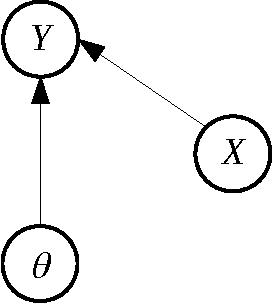
\includegraphics[width=.25\textwidth]{generative.pdf}\label{fig:generative}}
\hspace*{.2\textwidth}
\subfigure[Discriminative model]{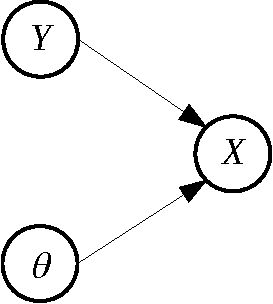
\includegraphics[width=.25\textwidth]{discriminative.pdf}\label{fig:discriminative}}
\caption{Bayesian networks representing generative and discriminative models, where $X$, $Y$ and $\theta$ respectively denote the variable of interest, the data, and the model parameters. Note the marginal independence of~$Y$ and~$\theta$ in the discriminative model.}
\label{fig:graph_comparison}
\end{center}
\end{figure}

Composite likelihood (CL, see \cite{Varin-11} and the references therein) is a semi-generative approach to statistical inference that extends the familiar notion of likelihood without requiring a full generative model. The key idea is to model an arbitrary set of low-dimensional features separately and then combine them, instead of modeling the data distribution as a whole. This may be viewed as a {\em divide and conquer} method to approximate the true but intractable likelihood. While maximum CL does not inherit the general property of maximum likelihood to yield an asymptotically minimum-variance estimator, it is consistent under mild conditions \cite{Xu-11} and may offer an excellent trade-off between computational and statistical efficiency in practice. 

In this note, CL is interpreted as a probabilistic opinion pool of ``agents'' making use of different pieces of information, or clues, extracted from the input data. Each agent acts as an isolated generative model-based statistician and expresses an opinion based on a single clue in the form of a likelihood function of the hidden variables. The agent opinions are then aggregated into a probability distribution on the hidden variables analogous to a Bayesian posterior.

We further argue that a particular log-linear opinion pool yields the best possible predictive distribution in the sense of maximum relative conditional entropy. This perspective entails a method to optimize the weights of the different agents from training data as in a typical discriminative learning scenario. 

%Something for true statisticians. Maybe we could clarify that we use the term ``Bayesian'' in the sense of ``empirical Bayesian'', implying that the parameters $\theta$ are to be estimated somehow contrary to a ``full Bayesian'' approach where they would be integrated out at inference time.


\section{Composite likelihood as opinion pooling}
\label{sec:pool}

Let $Y$ an observable multivariate random variable with sampling distribution $p(y|x)$ conditional on some unobserved variable of interest, $X\in{\cal X}$, where ${\cal X}$ is a known set. Given an experimental outcome $y$, the likelihood is the sampling distribution evaluated at $y$, seen as a function of $x$:
$$
L(x) = p(y|x)
.
$$

This requires a plausible generative model which, for complex data, may be out of reach or involve too many parameters to be estimated. A natural workaround known as {\em data reduction} is to extract some lower-dimensional representation $z=f(y)$, where $f$ is a many-to-one mapping, and consider the potentially more convenient likelihood function:
$$
\ell(x) = p(z|x)
.
$$

Substituting $L(x)$ with $\ell(x)$ boils down to restricting the sample space, thereby  ``delegating'' statistical inference to an ``agent'' provided with partial information. While it is valid for such an agent observing~$z$ only to consider $\ell(x)$ as the likelihood function of the problem, the drawback is that $\ell(x)$ might yield too vague a prediction of~$X$ due to the information loss incurred by data reduction. To make the trick statistically more efficient, we may extract several features, $z_i=f_i(y)$ for $i=1,2,\ldots,n$, and try to combine the likelihood functions $\ell_i(x) = p(z_i|x)$ that they elicit.

If we see the likelihoods as posterior distributions corresponding to uniform priors, this is a classical problem of probabilistic opinion aggregation from possibly redundant sources, for which several methods exist in the literature \cite{Tarantola-82,Genest-86,Garg-04,Allard-12}. We will show in Section~\ref{sec:maxent} that one that is particularly well-suited to our case is the {\em log-linear opinion pool}: 
\begin{equation}
\label{eq:log_pool}
p_\lambda(x|y) = \frac{1}{z_\lambda(y)} \pi(x) \prod_{i=1}^n p(z_i|x)^{\lambda_i},
\end{equation} 
where $\pi(x)$ is some reference distribution or prior, and $\lambda=(\lambda_1,\ldots,\lambda_n)$ is a vector of weights so that the normalizing factor:
$$
z_\lambda(y) = \int \pi(x) \prod_{i=1}^n p(z_i|x)^{\lambda_i} dx
$$
is finite, which holds whenever $\lambda\succeq 0$, {\em i.e.} all weights are positive, assuming that the agent opinions are always upper bounded. Negative weights should be ruled out as the existence condition $z_\lambda(y)<\infty$ would then depend on the particular opinions expressed by the agents. Also note that, while it is possible to have the weights depend on~$y$, there is a strong rational for constant weights as we shall see in the sequel. 

%Strictly positive weights guarantee the so-called 0/1 forcing property, that is, if an hypothesis~$x$ has zero likelihood according to at least one agent, then its consensus probability vanishes too.

% Not clear yet as to what a negative weight could mean!

The log-linear pool~(\ref{eq:log_pool}) bears a striking similarity to Bayes rule, yielding the form: $p_\lambda(x|y)\propto \pi(x) L^c_\lambda(x)$, where the quantity:
\begin{equation}
\label{eq:comp_lik}
L^c_\lambda(x) \equiv \prod_{i=1}^n \ell_i (x)^{\lambda_i}
\end{equation} 
plays the same role as a traditional likelihood function. This expression happens to be known in statistics as a {\em marginal composite likelihood} \cite{Varin-11}. See Appendix~\ref{sec:conditional} for the slightly more general form called {\em conditional composite likelihood}, which can be derived in the same way.

From~(\ref{eq:comp_lik}), we see that CL shares a convenient factorized form with the likelihood derived under the assumption of mutual feature independence, usually referred to as {\em na\"ive Bayes} or {\em simple Bayes} in the machine learning literature, which corresponds to the special case of unitary weights, $\lambda_1=\ldots=\lambda_n= 1$. The clear computational advantage of CL over the true likelihood is that it only requires to evaluate the marginal feature distributions rather than the joint distribution of all features.


\section{Tuning composite likelihood weights}

When the features can be considered exchangeable, it is natural to choose uniform CL weights. The CL is then a scaled version of the na\"ive Bayes likelihood, the common weight value being irrelevant to the maximum CL estimator (MCLE). The weight may be tuned so as to best adjust the pseudo posterior variance matrix to the asymptotic variance matrix of the MCLE \cite{Pauli-11}, or via a close-in-spirit curvature adjustment \cite{Ribatet-12}, in attempts to match the frequentist and composite Bayesian notions of uncertainty.

Ignoring such a goal, another frequent recommandation for CL weights is to sum up to one. This can be motivated in various ways. It turns out that the only pooling operator that does not explicitly depend on~$x$ and preserves {\em external Bayesianity} is the log-linear opinion pool with unit sum weights \cite{Genest-86b}. External Bayesianity essentially means that it should not matter whether the prior is incorporated before or after pooling, provided that all agents agree on the same prior. Another appealing property of log-linear pooling with unit sum weights is to minimize the average Kullback-Leibler (KL) divergence to the agent opinions \cite{Garg-04}. A maximum relative entropy property is also given in \cite{Wang-14}, Theorem~3.

Unit sum weights, however, correspond to the extreme situation where the features are assumed to be maximally redundant, but is clearly ineffective for independent or weakly correlated features, which require weights close to one for the CL to closely approximate the true likelihood. In this case, the CL may be much flatter than it should, leading to severly overestimated credibility sets.

{\color{red} Why is it important to fine-tune the weights?}
We therefore need a method to tune weights that can automatically adjust to the level of statistical dependence beween features.

%Instead, redundancy between agents is assumed by default, and is effectively encoded by the unit sum constraint on weights\footnote{Nevertheless, features which are {\em known} to be mutually independent can be merged into a single feature. This results in increasing their weights in the log-linear pool.}.

\section{Maxent composite likelihood}
\label{sec:maxent}

We can derive composite likelihood from the conditional maximum entropy principle \cite{BergerA-96}. It comes with a method of tuning weights, hence a particular composite likelihood function that we call maxent composite likelihood (MCL).

A cheap MaxEnt argument was already given by \cite{Wang-14}  (standard, non-conditional MaxEnt at fixed $y$, hence just an existence result but no feasible weight tuning).

What we do here is maximum {\em conditional} entropy. It's slightly more complex than a simple $I$-projection. The search space is a set of predictive distributions compatible with mean log-likelihood contraints. If I know the generative distribution, I know the expected log-likelihood.

We work with inequality constraints to force $\lambda\geq 0$:
$$
E[\log p(z_i|x)] \geq c_i \equiv \int \pi(x)p(z_i|x) \log p(z_i|x) dx dy
$$

What does the constraint mean? It means that a model is admissible if it compresses the data at least as well as all my agents. So we are not assuming that the generative models are {\em true}. We only assume that they are useful to compress the (reduced) data. Connection to MDL. 

Why not using the feature-based posteriors or Bayes factors rather than the likelihoods? It's a possibility (perhaps a connection here with Gr\"unwald's luckiness). A justification for not doing it is that the coordinator should discard the priors used by the agents. The constraints are not purely evidence-based since the moments depend on the coordinator's prior but it is arguable a mess of priors wouldn't be good.

Intuition behind weights: Lagrange multipliers to enforce a constraint... Notion of feature relevance. But does $\lambda_1>\lambda_2$ imply that $z_1$ is more relevant than $z_2$? 

The derivation assumed the marginal distribution of the data $h(y)$ to be known. In practice, it is estimated by the empirical distribution just like the moments are estimated.

Game theoretic interpretation \cite{Grunwald-04}.

The dual function boils down to the famous cross-entropy.

Single feature case ($y=z$): the maxent solution has the form $p(x|y)\propto\pi(x)p(y|x)^\lambda$. We expect to have $\lambda=1$ but it's not necessarily the case. It is if $h(y)=\int\pi(x)p(y|x)dx$ because then $h(y)p(x|y)=\pi(x)p(y|x)$ so the constraint is verified (and active). This also tells us that the data marginal should be consistent with the prior on labels for this much expected consistency property to hold. So, either weight datapoints so as to match a desired prior (e.g., uniform) or take the empirical distribution of labels as the ``prior''. 

Which brings another question: in this case, the (unique) weight is insensitive to the prior -- is it true in general? The answer is no. The weights generally depend on the prior. Hence the maxent composite likelihood is prior-dependent. This is an important conceptual difference with the classical notion of likelihood.

\section{Super composite likelihood}
\label{sec:super}

When chosen for computational simplicity, clues may not only convey limited information at individual level: their informativeness may also be very much hypothesis-dependent. Consider, for instance, diagnosing a disease from a routine medical checkup. Body temperature may point to a bacterial infection by comparison with normality, but would not help detecting a non-infectious cardiovascular disease -- and conversely for, say, blood pressure.

This motivates a more general setting where clues can be weighted differently depending on hypotheses.

What happens if we use mean-values constraints conditional on $x$ instead of jointly averaged over $x$ and $y$? This boils down to picking functions of the form:
$$
\chi(x-a)\ell_i(x,y)
$$

The answer is that the maxent solution has the form:
$$
p_\lambda(x|y) = \pi(x) \prod_i p(z_i|x)^{\lambda_i(x)}
$$

In other words, the weights become dependent on the variable of interest. This is the super composite likelihood idea.


\section{Composite EM algorithm for unsupervised learning}
\label{sec:gem}

In a nutshell: alternate unsupervised learning of partial model parameters ($M$-step) and re-estimation of label posteriors via maxent ($E$-step). 

$M$-step: given a posterior estimate $q(x|y)$, do just as if the features were independent and solve: 
$$
\max_\theta
\int \sum_i h(y)q(x|y) \log p_\theta(z_i,x) dx dy
$$

Note we can estimate cross-feature parameters such as class proportions.

Surrogate $E$-step: given generative parameters, recompute the moment constraints and update $q(x|y)$ according to the conditional maxent principle:
$$
\min_q
\int h(y)q(x|y) \log \frac{q(x|y)}{\pi(x)} dx dy
$$
s.t.
$$
\int h(y)q(x|y)\log p_\theta(z_i|x) dx dy \geq \int \pi(x)p_\theta(z_i|x)\log p_\theta(z_i|x) dx dy
$$

However, there is an important issue: how is $h(y)$ defined in both the $M$- and $E$-steps? In supervised context, $h(x,y)$ can be defined beforehand as the prior-corrected empirical distribution:
$$
h(x,y) = \pi(x) \frac{h_0(x,y)}{h_0(x)},
$$
where $h_0(x,y)$ is the raw empirical distribution. In unsupervised context, the best we can do is to replace $h_0(x,y)$ with $h_0(y)q(x|y)$, implying that the empirical distribution of $y$ is reweighted according to:
$$
h(y) = \sum_i w_i\delta(y-y_i),
\qquad
w_i = \int \pi(x)\frac{q(x|y_i)}{\sum_j q(x|y_j)} dx,
$$
which needs to be done each time $q(x|y)$ is updated, that is, after each $E$-step.

The other option is to keep $h(y)$ constant throughout the iterations but adapt $\pi(x)$ as the marginal distribution of labels learned in the $M$-step. In this case, it's no longer a ``prior''. 

Are we minimizing a unique functional as in the variational EM algorithm? Possibly not. We may see this generalization as a two-player game. One player tries to predict several data features independently. The other player tries to predict labels. Together, they find patterns (clusters) in unlabeled data. Does the more general version converge? Does the game have a value? And so on.

In the case of a single feature, is this the well-known EM? The $M$-step is clearly the same, what about the $E$-step? It is the same if $h(y)p_\theta(x|y)=p_\theta(y|x)\pi(x)$. However, this condition won't hold if $h(y)$ is an empirical distribution... In this special case, the ``E player'' could use the data distribution model produced by the ``M player'' instead of the empirical one but, more generally, there is no data distribution model so he has to stick to the empirical one.

The maxent is a surrogate for the $E$-step. It reflects the lack of a full model $p_\theta(x,y)$.

% Accounting here for Xi'An comment on xianblog.wordpress.com
% The sum of the powers is constrained to be equal to one, even though
% I do not understand why the dimensions of the projections play nog
% role in this constraint. Simplicity is advanced as an argument,
% which sounds rather weak…
%This simple constraint is implied by the external Bayesianity requirement: as it turns out, the only aggregation operator which is both externally Bayesian and independent from $x$ boils down to plugging a composite likelihood with unit sum weights into Bayes rule, hence extending the classical notion of likelihood in Bayesian analysis.


\section{Discussion}
\label{sec:discussion}

Deep learning is discriminative...

CL is a concept from computational statistics that has mainly been developed so far in a frequentist perspective as a surrogate for the maximum likelihood method. We have shown a deep connection between CL and probabilistic inference, thereby establishing CL as a class of discriminative models. Because CL is built from a set of marginal feature-specific generative distributions, it is in essence a two-step semi-generative, semi-discriminative learning approach. In the first, ``generative'' phase, the feature distributions are learned; in the second, ``discriminative'' phase, the feature weights are learned. This strategy can be thought of as a form of non-adaptive boosting.

%The first phase corresponds to the training of ``weak learners''. The second phase amounts to a form of boosting. 

A purely discriminative learning could be used instead but...
Why potentially more efficient than pure discriminative training: because generative training is always more efficient than discriminative training if models are comparable. So the key point is that ``we have less parameters in the discriminant phase". Good in small datasets. But also in asymptotic regime if the features are weakly or highly correlated (???).

Logistic regression / naive Bayes example. Under homoscedasticity (assuming that each feature has class-independent variance), CBI is equivalent to logistic regression -- because the predictive distribution family is the same. This is a case where BCI brings nothing. But consider heteroscedasticity, then BCI yields a quadratic classifier. Compared to a fully discriminative model, the number of parameters to learned in the discriminative phase is reduced by half.

The first training phase is easier if supervised but could be unsupervised too (using mixture models). How do we then deal with label switching issues? Can we safely assume conditional feature independence {\em in the generative training phase}? I believe so provided that the marginal distribution parameters are disjoint. It's obvious in the supervised learning scenario.

If unsupervised, the first learning phase could be compared with contrastive pre-training of RBMs \cite{Hinton-06,Fischer-14}, which also optimize parameters for generation of observable features. BCI is comparable with an RBM with a single output unit (which is just a generative model assuming conditionial feature independence). The key difference is that the RBM is a full generative model while BCI only deals with marginal models, hence relying on weaker assumptions. This won't change anything in the pre-training phase but RBMs have to deal with more parameters in the generative learning phase. In fully supervised context, RBM pre-training is pointless since all parameters learned in the first phase will be overwritten. In BCI, pre-training is crucial even in supervised context because the parameters learned in the discriminative phase (the feature weighs) describe a sub-manifold of the predictive distribution family.

Needs features. Not a representation learning method, but could be coupled why not.


%{\color{red} Moreover, while RBM parameters are typically refined in a supervised discriminative learning step, disjoint set of parameters for SCL. Dunno how to say that.} 

%In such context, SCL competes with classical discriminative models (logistic regression, Gaussian processes \cite{Rasmussen-06}, maximum entropy models \cite{BergerA-96}, etc.), and may compare more or less favorably in practice depending on the amount of training data. For relatively small training datasets, we may hope for more accurate inference using~SCL than using traditional discriminative models, extrapolating from the results of \cite{Ng-01} regarding the comparison between logistic regression and na\"ive Bayes classifiers.
%{\color{red}Ici, il manque la comparaison avec les RBMs qui ne sont pas (forcement) des modeles discriminatifs.}

%%, hence alleviating the need for heavily supervised model training

%In summary, CL has the potential to yield weakly supervised or unsupervised Bayesian-like inference procedures depending on the particular task at hand. This property reflects the encoding of statistical relationships between the data and {\em all} unknown parameters. CL thus appears as a trade-off between generative models, which are optimal for unsupervised learning but possibly intractable, and traditional discriminative models (logistic regression, Gaussian processes \cite{Rasmussen-06}, maximum entropy models \cite{BergerA-96}, etc.), which are inherently supervised. CL models are discriminative models assembled from atomic generative models and, from this point of view, may be considered as {\em semi-generative} models.

%CL may be considered as a {\em semi-generative} model: a discriminative model assembled from partial generative models.

%As a note of caution, we shall stress that the pre-determined weights assigned to the different associations between observed and unobserved values represent prior knowledge regarding the informativeness of clues. A poor choice of weights will inevitably result in a poor approximation to the ``true'' Bayesian posterior -- the posterior that would be obtained from a realistic generative model if it was tractable. In future work, we will investigate feature selection strategies to mitigate this problem.

% Improve the discussion on following aspects:
% ** Why is it compatible with unsupervised learning? Give more insight.
% ** Stress the contribution: class-specific weighting.
% * Pivotality argument.
% * Bayes is a special case of composite Bayes.

{\color{red}Product of fucking experts \cite{Hinton-02}. Log-linear pool to build a generative model (assuming in fact independence between experts). Better seen as a ``log-mixture model''. Sounds like each expert is associated with a class, so it's the same as a RBM. Contrastive learning approximates ML parameter estimation. The experts are learning jointly. It's just a generative model.}

{\color{red}Two-step training: generative phase then discriminative phase. Why is it cool?}

{\color{red}CBI is just a way to reweight Naive Bayes. What's the big deal? Can we really expect massively superior performance? Are we just talking about realistic credibility sets?}


\appendix

\section{Conditional composite likelihood}
\label{sec:conditional}

As a straightforward  extension of marginal CL, each feature-based likelihood may be conditioned by an additional ``independent'' feature $z^c_i = f^c_i(y)$ considered as a predictor of the ``dependent'' feature, $z_i=f_i(y)$, yielding the more general form:
\begin{equation}
\label{eq:cond_feat_lik}
\ell_i(x) = p(z_i|x,z^c_i).
\end{equation}

Conditioning may be useful if it is believed that $z^c_i$ alone is little or not informative about $x$, but can provide relevant information when considered jointly with $x$, as in the case of regression covariates, for instance. Equation~(\ref{eq:comp_lik}) then amounts to conditional CL \cite{Varin-11}, a more general form of CL also including Besag's historical {\em pseudo-likelihood} \cite{Besag-74} developed for image segmentation.


\section{Minimally discriminative model}

Let $\pi(x)$ some reference distribution that represents full
uncertainty about $X$. We wish to select the joint distribution
$p(x,y)$ that minimizes:
$$
I(p) = \int p(x,y) \log \frac{p(x|y)}{\pi(x)} dy,
$$ subject to feature mean-value constraints of the form:
$$
\int p(x,y) f(x,y) dx dy = \mu.
$$

There are two special cases of this problem in the literature.  On the
one hand, the {\em maximum entropy classifier} \cite{BergerA-96}
incorporates the constraint that $p(y)$ be known, however we will see
that this is not necessary. The {\em minimally informative likelihood}
method \cite{Yuan-99b,Yuan-99}, on the other hand, imposes that
$p(x)=\pi(x)$, hence assuming the form $p(x,y)=\pi(x)p(y|x)$. We won't
make such assumptions here and will consider the case where $\mu$ is
completely unknown.

The above problem is seen to be equivalent to minimizing the auxiliary
objective function:
$$
I(p,m) 
= \int p(x,y) \log \frac{p(x,y)}{\pi(x)m(y)} dxdy,
$$ over $p$ and $m$, subject to the same constraints on $p$. We note
that $I(p,m)=I(p)+D(p_y\|m)$, showing that the auxiliary function
essentially adds a penalty term to the actual objective in order to
force $p(y)$ close to $m(y)$.

Minimizing $I(p,m)$ along both $p$ and $m$ is basically a minimum KL
divergence problem between two convex distribution spaces, so there
must be a unique solution {\bf -- to be checked in
  \cite{Cover-91}}. It is similar to the rate-distortion problem in
information theory, which may be solved by alternate minimization,
yielding a Blahut-Arimoto algorithm.
\begin{itemize}
\item {\em Let's call it A-step}. Optimize $p(x,y)$ at fixed $m$
  s.t. constraint:
$$
\exists \lambda, \qquad
p_{\lambda,m}(x,y) = \frac{1}{Z(\lambda, m)} \pi(x) m(y) e^{-\lambda^\top t(x,y)}
$$
The actual $\lambda$ is found my maximizing the dual function
$\psi(\lambda,m)$, see below.
\item {\em Let's call it B-step}. Optimize $m(y)$ at fixed $p(x,y)$:
$$
m(y) = \int p(x,y) dx
$$
\end{itemize}

Upon convergence, the algorithm outputs both joint and marginal
distributions $p_{\star}(x,y)$ and $m_{\star}(y)$ that both depend on
$\mu$. By construction, we have that $p_{\star}(y) = m_{\star}(y)$,
therefore $p_\star(x|y)=p_{\star}(x,y)/m_{\star}(y)$.


\section{Comparison with maximum entropy classifier}

Lagrangian...
$$
{\cal L}(p,m,\lambda)
= 
\int p(x,y) \log \frac{p(x,y)}{\pi(x)m(y)} dxdy
+
\lambda^\top \left( 
\int p(x,y) f(x,y) dydy - \mu 
\right)
$$ where $\lambda$ represents a vector-valued Lagrange multiplier. At
fixed $m$, the solution has the form:
$$
p_{\lambda,m}(x,y) = \frac{1}{Z(\lambda,m)}
\pi(x) m(y) e^{-\lambda^\top f(x,y)} 
$$

Note that this implies that the conditional distribution is
independent of $m$ once $\lambda$ is determined,
$$
p_\lambda(x|y) = \frac{1}{z(\lambda,y)} \pi(x) e^{-\lambda^\top f(x,y)} 
$$

Also, the marginal is a modulation of $m(y)$:
$$
p_{\lambda,m}(y) = \frac{z(\lambda,y)}{Z(\lambda,m)} m(y)
$$

Dual function at fixed $m$:
$$
\psi(\lambda,m) 
\equiv \min_p {\cal L}(p,m,\lambda)
= 
- \log Z(\lambda,m) - \lambda^\top \mu
.
$$ 

An alternative expression is:
$$
\psi(\lambda, m)
= 
\int h(x,y) 
\log \frac{p_{\lambda,m}(x,y)}{\pi(x)m(y)} dxdy,
$$ where $h(x,y)$ is any distribution statisfying the
constraints. This shows that maximizing the dual function at fixed $m$
is essentially the same as minimizing the KL divergence
$D(h\|p_{\lambda,m})$ over $\lambda$, in other words fitting $h(x,y)$
by some distribution of the form $p_{\lambda,m}$. The fact that the
result does not depend on the particular $h(x,y)$ that is chosen, as
long as it satifies the constraint, is a general property of
exponential families.

We also have that the dual function associated with $I(p)$ reads:
\begin{eqnarray*}
\psi(\lambda) 
 & = & \min_m \psi(\lambda, m)\\
 & = & \int h(x,y) \log \frac{p_{\lambda}(x|y)}{\pi(x)} dxdy\\
 & = & -\int h(y) \log z(\lambda,y) dy - \lambda^\top \mu
\end{eqnarray*}

But, wait, that's exactly what we get in the maximum entropy
classifier! So, at the end of the day, we simply got an alternative
method to learn $\lambda$ in the maximum entropy classifier, i.e. the
Blahut-Arimoto algorithm as opposed to a brute-force maximization of
$\psi(\lambda)$. Both methods will converge to the same $\lambda$...

What it essentially means is that the optimal $\lambda$ is insensitive
to $m(y)$ as long as $m(y)$ is compliant in the sense that:
$$
m(y) = \int h(x,y) dx,
$$ for some distribution $h(x,y)$ statisfying the constraint. This is
true for the optimal $m_\star(y)$ output by the BA algorithm, but
also, for instance, for the empirical distribution of observations in
a training dataset used to estimate $\mu$, as proposed in
\cite{BergerA-96}. The only special property of $m_\star(y)$ is to
yield the full Bayesian model $p_\star(x,y)=p_\star(x|y)m_\star(y)$
that minimizes the discrimination information. We may not care too
much about that in practice since we will only use $p_\star(x|y)$. 

\section{Comparison with minimally informative likelihood}

Yuan \cite{Yuan-99} considered the situation where we add the
constraint that $p(x)=\pi(x)$ to the minimum discrimination inference
problem. Unknown is then the conditional distribution
$p(y|x)$. Lagrangian...
\begin{eqnarray*}
{\cal L}(p,m,\lambda)
 & = & 
\int \pi(x)p(y|x) \log \frac{p(y|x)}{m(y)} dxdy
+
\lambda^\top \left( 
\int \pi(x)p(y|x) f(x,y) dydy - \mu 
\right) \\
 & = & 
\int \pi(x)
\left( 
\int
p(y|x) \log \frac{p(y|x)}{m(y)} dy
+
\lambda^\top 
\int p(y|x) f(x,y) dy
- \mu 
\right)
dx 
\end{eqnarray*}

The derivative is given by,
$$
\frac{\partial\cal L}{\partial p(y|x)}
= 
\pi(x)\left[ 
1 + \log \frac{p(y|x)}{m(y)} 
+ \lambda^\top f(x,y)
\right],
$$
hence the optimal model at fixed $m$ has the form:
$$
p_{\lambda,m}(y|x) = \frac{1}{Z(\lambda,m,x)} m(y) e^{-\lambda^\top f(x,y)} 
$$

Note that the induced posterior distribution $p_{\lambda,m}(x|y)$ has
a different form from above unless the normalizing factor
$Z(\lambda,m,x)$ turns out independent from $x$. If this is not the
case, we no longer have the property that $p_{\lambda,m}(x|y)$ is
independent from $m$ given $\lambda$.

Dual function...
$$
\psi(\lambda,m) 
=
- \int \pi(x) \log Z(\lambda, m, x) dx
- \lambda^\top \mu
$$

Equivalently, for any distribution under the form $\pi(x)h(y|x)$ that
satisfies the moment constraint, we have:
$$
\psi(\lambda,m) 
=
\int \pi(x) h(y|x) \log \frac{p_{\lambda,m}(y|x)}{m(y)} dxdy
$$

Now, the real question is why should we constrain $p(x)$, which boils
down to a Bayesian prior in this context, to be the same as our
reference $\pi(x)$? It only makes sense if we want our inference to
stick to a generative modeling paradigm... but haven't we already
given up on that? Therefore, unless we find a good reason not to, we
won't impose the $p(x)=\pi(x)$ constraint, thereby allowing for a
discrepancy between the reference and the prior.


\section{Discriminative vs. semi-discriminative}

Let's go back to the equivalence we found between our approach and the
maximum entropy classifier (MCE) \cite{BergerA-96}. We have said that
the former is essentially a re-formulation of MCE.

But the re-formulation also conveys a generalization of MCE if,
instead of letting $m$ being an arbitrary distribution, we restrict
its search space to some set of acceptable reference
distributions. Would such a strategy be useful? 

Recall that the method selects the joint distribution that minimizes
discriminative information, as defined by $I(p)$:
$$
I(p) 
= \int p(x,y)\log\frac{p(x|y)}{\pi(x)} dxdy
= E_Y[D(p_{x|y}\|\pi)]
$$

The latter characterization reminds us that discriminative information
is defined in an average sense. The corresponding posterior $p(x|y)$
may not be conservative for some $y$, in particular those that are
unlikely under $p(y)$. It would be a problem if that's the case for
the particular data at hand. For that to happen rarely, the ideal
$p(y)$ would be the ``true'' marginal distribution of $Y$.

However, for vague mean value constraints, nothing may prevent the
optimal $m_\star(y)$ from departing significantly from that ideal
distribution. In fact, we can show that $m_\star(y)$ only has mass at
$y$ values that maximize $z(\lambda_\star,y)$, and is therefore likely
sparse. This is because $m_\star$ minimizes $\psi(\lambda_\star,m)$,
which is equivalent to maximizing $Z(\lambda_\star,m)$ and we have:
$$
Z(\lambda, m) = \int m(y) z(\lambda, y) dy.
$$

In other words, the solution to our problem may be singular! It does
not hurt since, as discussed above, one may alternatively fix $m(y)$
to some pre-defined distribution... but this, in practice, restricts
the method to supervised learning situations.

We may not face this issue with the MIL method, which further imposes
the prior on $X$, so all the information from the constraints goes
into specifying a possibly reasonable generative model.



\bibliographystyle{abbrv}
\bibliography{cvis,stat,alexis}

%%\input{draft.biblio}

\end{document}


\end{document}


\end{document}


\end{document}
